\subsection{CONJUGACY OF CARTAN SUBALGEBRAS OF SOLVABLE LIE ALGEBRAS}

Let g be a solvable Lie algebra. Denote by \(\mathcal{C}^{\infty}(\mathfrak{g})\) the intersection of the terms of the descending central series of g (Chap. I, §1, no. 5). This is a characteristic ideal of g, and is the smallest ideal m of g such that g/m is nilpotent. Since \(\mathcal{C}^{\infty}(\mathfrak{g}) \subset [\mathfrak{g}, \mathfrak{g}]\) , \(\mathcal{C}^{\infty}(\mathfrak{g})\) is a nilpotent ideal of g (Chap. I, §5, no. 3, Cor. 5 of Th. 1). By Prop. 1 of no. 1, the set of \(e^{ad x}\) , for \(x \in \mathcal{C}^{\infty}(\mathfrak{g})\) , is a subgroup of \(\operatorname{Aut}(\mathfrak{g})\) contained in the group of special automorphisms (Chap. I, §6, no. 8, Def. 6).

THEOREM 3. Let \(\mathfrak{g}\) be a solvable Lie algebra, and let \(\mathfrak{h},\mathfrak{h}'\) be Cartan subalgebras of \(\mathfrak{g}\) . There exists \(x\in \mathcal{C}^{\infty}(\mathfrak{g})\) such that \(e^{\mathrm{ad}x}\mathfrak{h} = \mathfrak{h}'\) .

We argue by induction on \(\dim \mathfrak{g}\) , the case where \(\mathfrak{g} = 0\) being trivial. Let \(\mathfrak{n}\) be a minimal non-zero commutative ideal of \(\mathfrak{g}\) . Let \(\varphi : \mathfrak{g} \to \mathfrak{g} / \mathfrak{n}\) be the canonical morphism. Then \(\varphi(\mathcal{C}^{\infty} \mathfrak{g}) = \mathcal{C}^{\infty}(\mathfrak{g} / \mathfrak{n})\) (Chap. I, §1, no. 5, Prop. 4). Since \(\varphi(\mathfrak{h})\) and \(\varphi(\mathfrak{h}')\) are Cartan subalgebras of \(\mathfrak{g} / \mathfrak{n}\) (§2, no. 1, Cor. 2 of Prop. 4), there exists, by the induction hypothesis, an \(x \in \mathcal{C}^{\infty}(\mathfrak{g})\) such that \(e^{\mathrm{ad} \varphi(x)}\varphi(\mathfrak{h}) = \varphi(\mathfrak{h}')\) . Replacing \(\mathfrak{h}\) by \(e^{\mathrm{ad} x}\mathfrak{h}\) , we can assume that \(\varphi(\mathfrak{h}) = \varphi(\mathfrak{h}')\) , in other words that

\[
\mathfrak {h} + \mathfrak {n} = \mathfrak {h} ^ {\prime} + \mathfrak {n}.
\]

Then \(\mathfrak{h}\) and \(\mathfrak{h}'\) are Cartan subalgebras of \(\mathfrak{h} + \mathfrak{n}\) . If \(\mathfrak{h} + \mathfrak{n} \neq \mathfrak{g}\) , the assertion to be proved follows from the induction hypothesis. Assume from now on that \(\mathfrak{h} + \mathfrak{n} = \mathfrak{h}' + \mathfrak{n} = \mathfrak{g}\) .

By the minimality of \(\mathfrak{n}\) , \([\mathfrak{g},\mathfrak{n}] = \{0\}\) or \([\mathfrak{g},\mathfrak{n}] = \mathfrak{n}\) . If \([\mathfrak{g},\mathfrak{n}] = \{0\}\) , then \(\mathfrak{n} \subset \mathfrak{h}\) and \(\mathfrak{n} \subset \mathfrak{h}'\) (§2, no. 1, Prop. 5), so \(\mathfrak{h} = \mathfrak{h} + \mathfrak{n} = \mathfrak{h}' + \mathfrak{n} = \mathfrak{h}'\) . It remains to consider the case where \([\mathfrak{g},\mathfrak{n}] = \mathfrak{n}\) , so \(\mathfrak{n} \subset \mathcal{C}^{\infty}(\mathfrak{g})\) . The ideal \(\mathfrak{n}\) is a simple \(\mathfrak{g}\) -module; since \(\mathfrak{g} = \mathfrak{h} + \mathfrak{n}\) , and since \([\mathfrak{n},\mathfrak{n}] = \{0\}\) , it follows that \(\mathfrak{n}\) is a simple \(\mathfrak{h}\) -module. If \(\mathfrak{h} \cap \mathfrak{n} \neq \{0\}\) , then \(\mathfrak{n} \subset \mathfrak{h}\) , so \(\mathfrak{g} = \mathfrak{h}\) and \(\mathfrak{h}' = \mathfrak{h}\) . Assume now that \(\mathfrak{h} \cap \mathfrak{n} = \{0\}\) . Then \(\mathfrak{g} = \mathfrak{h} \oplus \mathfrak{n}\) and hence \(\mathfrak{g} = \mathfrak{h}' \oplus \mathfrak{n}\) , since \(\mathfrak{h}\) and \(\mathfrak{h}'\) have the same dimension.

For all \(x \in h\) , let \(f(x)\) be the unique element of n such that \(x - f(x) \in \mathfrak{h}'\) ; if \(x, y \in h\) ,

\[
[ x, y ] - [ x, f (y) ] - [ f (x), y ] = [ x - f (x), y - f (y) ] \in \mathfrak {h} ^ {\prime},
\]

so \(f([x,y]) = [x,f(y)] + [f(x),y]\) . By §1, no. 3, Cor. of Prop. 9, there exists \(a \in \mathfrak{n}\) such that \(f(x) = [x,a]\) for all \(x \in \mathfrak{h}\) . We have \((\operatorname{ad}a)^2(\mathfrak{g}) \subset (\operatorname{ad}a)(\mathfrak{n}) = 0\) , so, for all \(x \in \mathfrak{h}\) ,

\[
e ^ {\operatorname{ad} a} x = x + [ a, x ] = x - f (x).
\]

Thus \(e^{\mathrm{ad}a}(\mathfrak{h}) = \mathfrak{h}'\) . Since \(a \in \mathcal{C}^{\infty}(\mathfrak{g})\) , this completes the proof.

Lemma 3. Let g be a Lie algebra, r its radical, \(\varphi\) the canonical homomorphism from g to g/r, v an elementary automorphism of g/r. There exists an elementary automorphism u of g such that \(\varphi \circ u = v \circ \varphi\) .

We can assume that \(v\) is of the form \(e^{\mathrm{ad}b}\) , where \(b \in \mathfrak{g} / \mathfrak{r}\) and \(\mathrm{ad}b\) is nilpotent. Let \(\mathfrak{s}\) be a Levi subalgebra of \(\mathfrak{g}\) (Chap. I, §6, no. 8, Def. 7) and let \(a\) be the element of \(\mathfrak{s}\) such that \(\varphi(a) = b\) . Since \(\mathrm{ad}_{\mathfrak{s}}a\) is nilpotent, \(\mathrm{ad}_{\mathfrak{g}}a\) is nilpotent (Chap. I, §6, no. 3, Cor. of Prop. 3), and \(u = e^{\mathrm{ad}_{\mathfrak{g}}a}\) is an elementary automorphism of \(\mathfrak{g}\) such that \(\varphi \circ u = v \circ \varphi\) .

PROPOSITION 5. Let g be a Lie algebra, r its radical, h and h' Cartan subalgebras of g, and \(\varphi\) the canonical homomorphism from g to g/r. The following conditions are equivalent:

\begin{enumerate}
\def\labelenumi{(\roman{enumi})}
\item
  \(\mathfrak{h}\) and \(\mathfrak{h}'\) are conjugate by an elementary automorphism of \(\mathfrak{g}\) ;
\item
  \(\varphi (\mathfrak{h})\) and \(\varphi (\mathfrak{h}^{\prime})\) are conjugate by an elementary automorphism of \(\mathfrak{g} / \mathfrak{r}\) .
\item
  \(\Longrightarrow\) (ii): This is clear.
\item
  \(\Longrightarrow\) (i): We assume that condition (ii) is satisfied and prove (i). By Lemma 3, we are reduced to the case where \(\varphi(\mathfrak{h}) = \varphi(\mathfrak{h}')\) . Put \(\mathfrak{k} = \mathfrak{h} + \mathfrak{r} = \mathfrak{h}' + \mathfrak{r}\) , which is a solvable subalgebra of \(\mathfrak{g}\) . Then \(\mathfrak{h}\) and \(\mathfrak{h}'\) are Cartan subalgebras of \(\mathfrak{k}\) , so there exists \(x \in \mathcal{C}^{\infty}(\mathfrak{k})\) such that \(e^{\mathrm{ad}_{\mathfrak{k}}x}\mathfrak{h} = \mathfrak{h}'\) (Th. 3). Since \(\mathfrak{k}/\mathfrak{r}\) is nilpotent, \(\mathcal{C}^{\infty}(\mathfrak{k}) \subset \mathfrak{r}\) ; on the other hand, \(\mathcal{C}^{\infty}(\mathfrak{k}) \subset [\mathfrak{k},\mathfrak{k}] \subset [\mathfrak{g},\mathfrak{g}]\) , so \(x \in \mathfrak{r} \cap [\mathfrak{g},\mathfrak{g}]\) ; by Chap. I, §5, no. 3, Th. 1, \(\mathrm{ad}_{\mathfrak{g}}x\) is nilpotent, so \(e^{\mathrm{ad}_{\mathfrak{g}}x}\) is an elementary automorphism of \(\mathfrak{g}\) transforming \(\mathfrak{h}\) to \(\mathfrak{h}'\) .
\end{enumerate}

\subsection{LIE GROUP CASE}

PROPOSITION 6. Assume that k is R, C or a non-discrete complete ultrametric field of characteristic 0. Let G be a finite dimensional Lie group over k, e its identity element, g its Lie algebra, h a Cartan subalgebra of g, \(h_{r}\) the set of regular elements of g belonging to h.

\begin{enumerate}
\def\labelenumi{(\roman{enumi})}
\item
  Let \(\mathfrak{s}\) be a vector space complement of \(\mathfrak{h}\) in \(\mathfrak{g}\) , \(\mathfrak{s}_0\) a neighbourhood of 0 in \(\mathfrak{s}\) on which an exponential map is defined, and \(h_0 \in \mathfrak{h}_r\) . The map \((s, h) \mapsto \mathrm{F}(s, h) = (\exp \operatorname{ad} s).h\) from \(\mathfrak{s}_0 \times \mathfrak{h}\) to \(\mathfrak{g}\) is étale at \((0, h_0)\) .
\item
  The map \((g,h)\mapsto \mathrm{F}'(g,h) = (\operatorname {Ad}g).h\) from \(\mathbf{G}\times \mathfrak{h}_r\) to \(\mathfrak{g}\) is a submersion. In particular, its image \(\Omega\) is open. For all \(x\in \Omega\) , \(\mathfrak{g}^0 (x)\) is a Cartan subalgebra of \(\mathfrak{g}\) conjugate to \(\mathfrak{h}\) under \(\operatorname {Ad}(\mathrm{G})\)
\item
  Let \(h_0 \in \mathfrak{h}_r\) . For any neighbourhood \(\mathrm{U}\) of \(e\) in \(\mathrm{G}\) , the set \(\bigcup_{a \in \mathrm{U}} (\mathrm{Ad}a)(\mathfrak{h}_r)\) is a neighbourhood of \(h_0\) in \(\mathfrak{g}\) .
\end{enumerate}

Let \(h_0\) and \(\mathfrak{s}\) be as in (i). Let \(\mathrm{T}\) be the tangent linear map of \(\mathrm{F}\) at \((0, h_0)\) . Then \(\mathrm{F}(0, h) = h\) for all \(h \in \mathfrak{h}\) , so \(\mathrm{T}(0, h) = h\) for all \(h \in \mathfrak{h}\) . On the other hand, for \(\mathfrak{s}_0\) sufficiently small, the tangent linear map at 0 of the map \(s \mapsto \exp s\) from \(\mathfrak{s}_0\) to \(\operatorname{End}(\mathfrak{g})\) is the map \(s \mapsto \operatorname{ad}s\) from \(\mathfrak{s}\) to \(\operatorname{End}(\mathfrak{g})\) . Thus \(\mathrm{T}(s, 0) = [s, h_0]\) for all \(s \in \mathfrak{s}\) . Now the map from \(\mathfrak{g}/\mathfrak{h}\) to \(\mathfrak{g}/\mathfrak{h}\) induced by \(\operatorname{ad}h_0\) by passage to the quotient is bijective. It follows that \(\mathrm{T}\) is bijective, hence (i). Since \(\exp s = \operatorname{Ad}\exp s\) for all \(s \in \mathfrak{s}\) sufficiently close to 0, (iii) and the first assertion of (ii) follow. Every \(x \in \Omega\) is of the form \((\operatorname{Ad}a)(h)\) with \(a \in G\) and \(h \in \mathfrak{h}_r\) , so \(\mathfrak{g}^0(x) = (\operatorname{Ad}a)(\mathfrak{g}^0(h)) = (\operatorname{Ad}a)(\mathfrak{h})\) is a subalgebra of \(\mathfrak{g}\) conjugate to \(\mathfrak{h}\) under \(\operatorname{Ad}(G)\) .

\section{REGULAR ELEMENTS OF A LIE GROUP}

In nos. 1, 2 and 3 of this paragraph, we assume that k is R, C or a non-discrete complete ultrametric field of characteristic 0. We denote by G a finite dimensional Lie group over k, by g its Lie algebra, and by e its identity element. If \(a \in G\) , we denote by \(\mathfrak{g}^{1}(a)\) the nilspace of \(\operatorname{Ad}(a) - 1\) , in other words the space \(\mathfrak{g}^{1}(\operatorname{Ad}(a))\) (cf.~§1, no. 1).

\subsection{REGULAR ELEMENTS FOR A LINEAR REPRESENTATION}

Lemma 1. Let M be an analytic manifold over k and \(a = (a_{0}, \ldots, a_{n-1}, a_{n} = 1)\) a sequence of analytic functions on M. For all \(x \in M\) , let \(r_{a}(x)\) be the upper bound of those \(i \in [0, n]\) such that \(a_{j}(x) = 0\) for j \textless{} i and let \(r_{a}^{0}(x)\) be the upper bound of those \(i \in [0, n]\) such that \(a_{j}\) is zero on a neighbourhood of x for j \textless{} i.

\begin{enumerate}
\def\labelenumi{(\roman{enumi})}
\item
  The function \(r_a\) is upper semi-continuous.
\item
  For all \(x \in \mathrm{M}\) , \(r_a^0(x) = \liminf_{y \to x} r_a(y)\) .
\item
  The function \(r_a^0\) is locally constant.
\item
  The set of points \(x \in M\) such that \(r_{a}^{0}(x) = r_{a}(x)\) is the set of points of M on a neighbourhood of which \(r_{a}\) is constant. This is a dense open subset of M. If k = C and M is finite dimensional and connected, it is open and connected.
\item
  If \(r_a(x) = i\) , then \(a_i(x) \neq 0\) and, for all \(y\) in a neighbourhood of \(x\) , we have \(a_i(y) \neq 0\) , so \(r_a(y) \leq i\) .
\item
  If \(r_{a}^{0}(x) = i\) , the functions \(a_{0}, \ldots, a_{i-1}\) are zero on a neighbourhood of x and, for any y in this neighbourhood, \(r_{a}(y) \geq i\) . Consequently, \(\liminf_{y \to x} r_{a}(y) \geq i\) . Every neighbourhood of x contains a point y such that \(a_{i}(y) \neq 0\) and hence \(r_{a}(y) \leq i\) . Thus \(\liminf_{y \to x} r_{a}(y) = i\) .
\item
  Let \(i = r_a^0 (x)\) and let \(V\) be a neighbourhood of \(x\) such that \(a_{j}(y) = 0\) for all \(y\in V\) and all \(j < i\) . Then \(x\in M - Z\) , where \(Z\) denotes the set of points of \(M\) in a neighbourhood of which the function \(a_{i}\) is zero. Since \(Z\) is closed in \(M\) (Differentiable and Analytic Manifolds, Results, 5.3.5), \(V\cap (M - Z)\) is a neighbourhood of \(x\) . For every point \(y\) in this neighbourhood, \(r_a^0 (y) = i\) .
\item
  The function \(r_{a}-r_{a}^{0}\) is upper semi-continuous and its value at any point is \(\geq0\) . If \(r_{a}(x)=r_{a}^{0}(x)\) , \(r_{a}-r_{a}^{0}\) is zero on a neighbourhood of x, which shows that \(r_{a}\) is constant on a neighbourhood of x by (iii). Conversely, if \(r_{a}\) is constant on a neighbourhood of x, then \(r_{a}^{0}(x)=r_{a}(x)\) by (ii). The set of points \(x\in M\) such that \(r_{a}^{0}(x)=r_{a}(x)\) is thus an open subset \(\Omega\) of M. If \(x\in M\) and if \(r_{a}^{0}(x)<r_{a}(x)\) , every neighbourhood of x contains a point y such that \(r_{a}(y)<r_{a}(x)\) and \(r_{a}^{0}(y)=r_{a}^{0}(x)\) . Every neighbourhood of x thus contains a point y such that
\end{enumerate}

\[
r _ {a} (y) - r _ {a} ^ {0} (y) <   r _ {a} (x) - r _ {a} ^ {0} (x).
\]

It follows that \(\Omega\) is dense in M.

If M is connected and if p is the value of \(r_{a}^{0}\) on M, the points of \(\Omega\) are the points \(x \in M\) such that \(a_{p}(x) \neq 0\) . If k = C, this implies that \(\Omega\) is connected by Lemma 3 of Appendix II.

Let \(\rho\) be an analytic linear representation of \(G\) on a vector space \(V\) of finite dimension \(n\) over \(k\) . Put

\[
\det (\mathrm{T} - \rho (g) + 1) = a _ {0} (g) + a _ {1} (g) \mathrm{T} + \dots + a _ {n - 1} (g) \mathrm{T} ^ {n - 1} + \mathrm{T} ^ {n}.
\]

The functions \(r_a\) and \(r_a^0\) associated to the sequence \((a_0, a_1, \ldots, a_{n-1}, 1)\) will be denoted by \(r_\rho\) and \(r_\rho^0\) , respectively. Then, for all \(g \in G\) ,

\[
\begin{array}{l} r _ {\rho} (g) = \dim \mathrm{V} ^ {1} (\rho (g)) \\ r _ {\rho} ^ {0} (g) = \liminf _ {g ^ {\prime} \to g} \dim \mathrm{V} ^ {1} (\rho (g ^ {\prime})). \end{array}
\]

Lemma 2. Let \(0 \to V' \to V \to V'' \to 0\) be an exact sequence of G-modules defined by analytic linear representations \(\rho', \rho, \rho''\) of G, respectively. Then:

\[
r _ {\rho} = r _ {\rho^ {\prime}} + r _ {\rho^ {\prime \prime}}, \text { and } r _ {\rho} ^ {0} = r _ {\rho^ {\prime}} ^ {0} + r _ {\rho^ {\prime \prime}} ^ {0}.
\]

Indeed, for all \(g \in \mathbf{G}\) , there is (§1, no. 1, Cor. 3 of Th.1) an exact sequence

\[
0 \to (\mathrm{V} ^ {\prime}) ^ {1} (\rho^ {\prime} (g)) \to \mathrm{V} ^ {1} (\rho (g)) \to (\mathrm{V} ^ {\prime \prime}) ^ {1} (\rho^ {\prime \prime} (g)) \to 0,
\]

which proves the first assertion. The second follows from it since, by Lemma 1 (iv), \(r_{\rho}^{0} = r_{\rho}, r_{\rho'}^{0} = r_{\rho'}\) and \(r_{\rho''}^{0} = r_{\rho''}\) on a dense open subset of G.

DEFINITION 1. An element \(g \in \mathbf{G}\) is called regular for the linear representation \(\rho\) if \(r_{\rho}(g) = r_{\rho}^{0}(g)\) .

PROPOSITION 1. The regular points for an analytic linear representation \(\rho\) of G are the points of G in a neighbourhood of which \(r_{\rho}\) is constant. They constitute a dense open subset of G. If k = C and G is connected, the set of regular points for \(\rho\) is connected.

This follows from Lemma 1 (iv).

Remark. Let \(G^{*}\) be an open subgroup of G. An element \(a \in G^{*}\) is a regular element of G for the linear representation \(\rho\) of G if and only if it is a regular element of \(G^{*}\) for the linear representation \(\rho|G^{*}\) .

\subsection{REGULAR ELEMENTS OF A LIE GROUP}

DEFINITION 2. An element of G is said to be regular if it is regular for the adjoint representation of G.

In other words (Prop. 1), an element \(g \in \mathbf{G}\) is regular if, for all elements \(g'\) in a neighbourhood of \(g\) in \(\mathbf{G}\) , the dimension of the nilspace of \(\operatorname{Ad}(g') - 1\) is equal to the dimension of the nilspace of \(\operatorname{Ad}(g) - 1\) .

PROPOSITION 2. Let G' be a finite dimensional Lie group over k and f an open morphism from G to G'. The image under f of a regular element of G is a regular element of G'. If the kernel of f is contained in the centre of G, an element \(g \in G\) is regular if and only if \(f(g)\) is regular.

Indeed, let \(\mathfrak{g}'\) be the Lie algebra of \(G'\) and \(\mathfrak{h}\) the ideal in \(\mathfrak{g}\) given by the kernel of \(Tf|\mathfrak{g}\) . Let \(\rho\) be the linear representation of \(G\) on \(\mathfrak{h}\) defined by \(\rho(g) = \operatorname{Ad} g|\mathfrak{h}\) for all \(g \in G\) , and let \(\operatorname{Ad} \circ f\) be the linear representation of \(G\) on \(\mathfrak{g}'\) given by the composite of \(f\) with the adjoint representation of \(G'\) . These linear representations define an exact sequence of \(G\) -modules:

\[
0 \to \mathfrak {h} \to \mathfrak {g} \to \mathfrak {g} ^ {\prime} \to 0.
\]

By Lemma 2, \(r_{\mathrm{Ad}} = r_{\rho} + r_{\mathrm{Ad}\circ f}\) . Since \(r_{\mathrm{Ad}\circ f} = r_{\mathrm{Ad}}\circ f\) and since \(f\) is an open map, \(r_{\mathrm{Ad}\circ f}^{0} = r_{\mathrm{Ad}}^{0}\circ f\) . Consequently:

\[
r _ {\mathrm{Ad}} - r _ {\mathrm{Ad}} ^ {0} = r _ {\rho} - r _ {\rho} ^ {0} + \left(r _ {\mathrm{Ad}} - r _ {\mathrm{Ad}} ^ {0}\right) \circ f.
\]

Thus, if g is regular, \((r_{\mathrm{Ad}} - r_{\mathrm{Ad}}^{0})(f(g)) = 0\) , which means that \(f(g)\) is regular. If the kernel of f is contained in the centre of G,

\[
r _ {\rho} (g) = r _ {\rho} ^ {0} (g) = \dim \mathfrak {h}
\]

for all \(g \in G\) . Consequently, if \(f(g)\) is regular, \(r_{\mathrm{Ad}}(g) = r_{\mathrm{Ad}}^{0}(g)\) , in other words, g is regular.

PROPOSITION 3. Let \(G_{1}\) and \(G_{2}\) be two finite dimensional Lie groups over k. An element \((g_{1}, g_{2})\) of \(G_{1} \times G_{2}\) is regular if and only if \(g_{1}\) and \(g_{2}\) are regular elements of \(G_{1}\) and \(G_{2}\) , respectively.

The condition is necessary by Prop. 2. We show that it is sufficient. For all \(g = (g_{1}, g_{2}) \in \mathrm{G}_{1} \times \mathrm{G}_{2}\) , \(r_{\mathrm{Ad}}(g) = r_{\mathrm{Ad}}(g_{1}) + r_{\mathrm{Ad}}(g_{2})\) . In view of Lemma 1 (ii), it follows that \(r_{\mathrm{Ad}}^{0}(g) = r_{\mathrm{Ad}}^{0}(g_{1}) + r_{\mathrm{Ad}}^{0}(g_{2})\) . If \(g_{1}\) and \(g_{2}\) are regular, \(r_{\mathrm{Ad}}^{0}(g_{1}) = r_{\mathrm{Ad}}(g_{1})\) and \(r_{\mathrm{Ad}}^{0}(g_{2}) = r_{\mathrm{Ad}}(g_{2})\) , so \(r_{\mathrm{Ad}}^{0}(g) = r_{\mathrm{Ad}}(g)\) , which means that \(g\) is regular.

Lemma 3. Let \(a \in \mathbf{G}\) and let \(\mathfrak{m}\) be a complement of \(\mathfrak{g}^1(a)\) in \(\mathfrak{g}\) . Let \(\mathbf{U}\) be a neighbourhood of 0 in \(\mathfrak{g}\) and exp an exponential map from \(\mathbf{U}\) to \(\mathbf{G}\) . The map

\[
f: (x, y) \mapsto (\exp y) a (\exp x) (\exp y) ^ {- 1}
\]

from \((\mathfrak{g}^1 (a)\times \mathfrak{m})\cap \mathrm{U}\) to G is étale at \((0,0)\) .

The tangent linear maps at 0 of the maps \(x \mapsto a(\exp x)\) and \(y \mapsto (\exp y)a(\exp y)^{-1}\) are the maps \(x \mapsto ax\) and \(y \mapsto ya - ay = a(a^{-1}ya - y)\) from \(\mathfrak{g}\) to \(T_aG = ag\) (Chap. III, §3, no. 12, Prop. 46). Consequently, the tangent map of \(f\) at \((0,0)\) is the map \((x,y) \mapsto ax + a(a^{-1}ya - y) = a(x + a^{-1}ya - y)\) from \(\mathfrak{g}^1(a) \times \mathfrak{m}\) to \(ag\) . This map is injective. Indeed, if \(x \in \mathfrak{g}^1(a), y \in \mathfrak{m}\) and if \(x + a^{-1}ya - y = 0\) , then \((\mathrm{Ad}(a) - 1)y = \mathrm{Ad}(a)x \in \mathfrak{g}^1(a)\) since \(\mathrm{Ad}(a)\mathfrak{g}^1(a) \subset \mathfrak{g}^1(a)\) . This implies that \(y \in \mathfrak{g}^1(a)\) and consequently that \(y = 0\) . Since \(\mathrm{Ad}(a)\) is injective on \(\mathfrak{g}^1(a)\) , it follows that \(x = 0\) . Since \(\dim \mathfrak{g} = \dim \mathfrak{g}^1(a) + \dim \mathfrak{m}\) , this shows that \(f\) is étale at \((0,0)\) .

PROPOSITION 4. Let \(a \in G\) and \(H\) be a Lie subgroup germ of \(G\) with Lie algebra \(\mathfrak{g}^1(a)\) . The map \((b, c) \mapsto cabc^{-1}\) from \(H \times G\) to \(G\) is a submersion at \((e, e)\) .

Indeed, let \(\mathfrak{m}\) be a complement of \(\mathfrak{g}^1(a)\) in \(\mathfrak{g}\) and exp an exponential map of \(G\) defined on an open neighbourhood \(U\) of \(0\) in \(\mathfrak{g}\) . We can choose \(U\) so that \(\exp(U \cap \mathfrak{g}^1(a)) \subset H\) . The map \(f: (x, y) \mapsto (\exp x, \exp y)\) is an analytic map on a neighbourhood of \((0, 0)\) in \(\mathfrak{g}^1(a) \times \mathfrak{m}\) with values in \(H \times G\) . By Lemma 3, the composite of \(f\) with the map \(\varphi: (b, c) \mapsto cabc^{-1}\) is étale at \((0, 0)\) . It follows that \(\varphi\) is a submersion at \(f(0, 0) = (e, e)\) .

PROPOSITION 5. Let \(a \in G\) and let \(W\) be a neighbourhood of \(e\) in \(G\) . There exists a neighbourhood \(V\) of \(a\) with the following property: for all \(a' \in V\) , there exists an element \(g \in W\) such that \(\mathfrak{g}^1(a') \subset \mathrm{Ad}(g)\mathfrak{g}^1(a)\) .

Put \(\mathfrak{g}^1 = \mathfrak{g}^1(a)\) and let \(\mathfrak{g} = \mathfrak{g}^1 + \mathfrak{g}^+\) be the Fitting decomposition of \(\operatorname{Ad}(a) - 1\) (§1, no. 1). Let H be a Lie subgroup germ of G with Lie algebra \(\mathfrak{g}^1\) . For all \(h \in \mathrm{H}\) , \(\operatorname{Ad}(h)\mathfrak{g}^1 \subset \mathfrak{g}^1\) . Since \([\mathfrak{g}^1, \mathfrak{g}^+] \subset \mathfrak{g}^+\) , there exists a neighbourhood U of \(e\) in H such that \(\operatorname{Ad}(h)\mathfrak{g}^+ \subset \mathfrak{g}^+\) for all \(h \in \mathrm{H}\) . Since the restriction of \(\operatorname{Ad}(a)-1\) to \(g^{+}\) is bijective, U can be chosen so that the restriction of \(\operatorname{Ad}(ah)-1\) to \(g^{+}\) is bijective for all \(h\in U\) . Then \(\mathfrak{g}^{1}(ah)\subset\mathfrak{g}^{1}(a)=\mathfrak{g}^{1}\) for all \(h\in U\) . By Proposition 4, \(\operatorname{Int}(\mathrm{W})(a\mathrm{U})\) is a neighbourhood of a in G. If \(a'\in\operatorname{Int}(\mathrm{W})(a\mathrm{U})\) , then \(a'=g(ah)g^{-1}\) with \(g\in W\) and \(h\in U\) ; it follows that \(\mathfrak{g}^{1}(a')=\operatorname{Ad}(g)\mathfrak{g}^{1}(ah)\subset\operatorname{Ad}(g)\mathfrak{g}^{1}(a)\) .

COROLLARY. Let \(G^{*}\) be an open subgroup of G. If \(a \in G\) is regular, there exists a neighbourhood V of a such that, for all \(a' \in V\) , \(\mathfrak{g}^{1}(a')\) is conjugate to \(\mathfrak{g}^{1}(a)\) under \(\mathrm{Ad}(\mathrm{G}^{*})\) .

\subsection{RELATIONS WITH REGULAR ELEMENTS OF THE LIE ALGEBRA}

PROPOSITION 6. Let V be an open subgroup of g and let exp : V → G be an exponential map defined on V.

\begin{enumerate}
\def\labelenumi{(\roman{enumi})}
\item
  There exists a neighbourhood \(\mathrm{W}\) of 0 in \(\mathrm{V}\) such that \(\mathfrak{g}^1(\exp x) = \mathfrak{g}^0(x)\) for all \(x \in \mathrm{W}\) .
\item
  If \(k = \mathbf{R}\) or \(\mathbf{C}\) , \(\mathfrak{g}^1(\exp x) \supset \mathfrak{g}^0(x)\) for all \(x \in \mathfrak{g}\) .
\end{enumerate}

By Cor. 3 of Prop. 8 of Chap. III, §4, no. 4, there exists a neighbourhood \(V'\) of 0 in \(V\) such that, for all \(x \in V'\) , \(\exp(\mathrm{ad}(x)) = \sum_{n=0}^{\infty} \frac{1}{n!} \mathrm{ad}(x)^n\) is defined and \(\mathrm{Ad}(\exp(x)) = \exp(\mathrm{ad}(x))\) . If \(P \in k[X]\) and \(\alpha \in \mathrm{End}(\mathfrak{g})\) , it is easy to check that \(\mathfrak{g}^\lambda(\alpha) \subset \mathfrak{g}^{P(\lambda)}(P(\alpha))\) for all \(\lambda \in k\) . Consequently,

\[
\mathfrak {g} ^ {0} (\operatorname{ad} (x)) \subset \mathfrak {g} ^ {1} (\exp (\operatorname{ad} (x))) = \mathfrak {g} ^ {1} (\operatorname{Ad} (\exp x)) = \mathfrak {g} ^ {1} (\exp x)
\]

for all \(x \in V'\) . If k = R or C, V = g and we can take \(V' = V\) , which proves (ii). We prove (i). Let U be a neighbourhood of 0 in \(\text{End}(\mathfrak{g})\) such that \(\text{Log}(1 + \alpha) = \sum_{n > 0} (-1)^{n+1} \frac{1}{n} \alpha^n\) is defined for all \(\alpha \in U\) . Then \(\log \circ \exp = 1\) on a neighbourhood of 0 and \(\mathfrak{g}^1(1 + \alpha) \subset \mathfrak{g}^0 (\text{Log}(1 + \alpha))\) for all \(\alpha \in U\) . Let W be the neighbourhood of 0 in g consisting of those \(x \in V'\) such that \(\exp x \in 1 + U\) and

\[
\operatorname{Log} (\exp (\operatorname{ad} (x))) = \operatorname{ad} (x).
\]

Then, for all \(x \in W\) ,

\[
\begin{array}{c} \mathfrak {g} ^ {1} (\exp x) = \mathfrak {g} ^ {1} (\mathrm{Ad} (\exp x)) = \mathfrak {g} ^ {1} (\exp (\mathrm{ad} (x))) \\ \qquad \subset \mathfrak {g} ^ {0} (\operatorname{Log} (\exp (\operatorname{ad} (x)))) = \mathfrak {g} ^ {0} (\operatorname{ad} (x)) = \mathfrak {g} ^ {0} (x). \end{array}
\]

This shows that \(\mathfrak{g}^1 (\exp x) = \mathfrak{g}^0 (x)\) for all \(x\in \mathrm{W}\) .

Lemma 4. Let U be a neighbourhood of 0 in g and exp an exponential map from U to G, étale at every point of U and such that \(\mathfrak{g}^{1}(\exp x) = \mathfrak{g}^{0}(x)\) for all \(x \in U\) .

\begin{enumerate}
\def\labelenumi{(\roman{enumi})}
\item
  The function \(r_{\mathrm{Ad}}^0\) is constant and equal to the rank of \(\mathfrak{g}\) on \(\exp(\mathrm{U})\) .
\item
  If \(x \in \mathrm{U}\) , exp \(x\) is regular if and only if \(x\) is a regular element of \(\mathfrak{g}\) .
\item
  An element \(a \in \exp(\mathrm{U})\) is regular if and only if \(\mathfrak{g}^1(a)\) is a Cartan subalgebra of \(\mathfrak{g}\) .
\end{enumerate}

Let \(l = \operatorname{rk}(\mathfrak{g})\) . If \(x \in \mathrm{U}\) is a regular element of \(\mathfrak{g}\) ,

\[
r _ {\mathrm{Ad}} (\exp x) = \dim \mathfrak {g} ^ {1} (\exp x) = \dim \mathfrak {g} ^ {0} (x) = l.
\]

Since the regular elements of g belonging to U constitute a neighbourhood of x and exp is étale at x, this shows that exp x is regular and that \(r_{\mathrm{Ad}}^{0}(\exp x) = l\) . The regular elements of g belonging to U being dense in U, we have \(r_{\mathrm{Ad}}^{0}(a) = l\) for all \(a \in \exp(\mathrm{U})\) . Let \(a \in \exp(\mathrm{U})\) be a regular element of G and let \(x \in U\) be such that \(a = \exp x\) . Since \(\mathfrak{g}^{0}(x) = \mathfrak{g}^{1}(a)\) , \(\dim \mathfrak{g}^{0}(x) = r_{\mathrm{Ad}}^{0}(a) = l\) . Consequently, x is a regular element of g and \(\mathfrak{g}^{1}(a)\) is a Cartan subalgebra of g. Finally, if \(a \in \exp(\mathrm{U})\) and \(\mathfrak{g}^{1}(a)\) is a Cartan subalgebra of g,

\[
r _ {\mathrm{Ad}} (a) = \dim \mathfrak {g} ^ {1} (a) = l = r _ {\mathrm{Ad}} ^ {0} (a),
\]

so \(a\) is regular.

PROPOSITION 7. Let V be a neighbourhood of e in G. Every Cartan sub-algebra of g is of the form \(\mathfrak{g}^{1}(a)\) where a is a regular element of G belonging to V.

By Prop. 6, there exists an open neighbourhood U of 0 in g and an exponential map \(\exp: U \to G\) satisfying the conditions of Lemma 4. If h is a Cartan subalgebra of g, there exists a regular element \(x \in h\) such that \(\mathfrak{h} = \mathfrak{g}^{0}(x)\) (§3, Th. 2). On the other hand, there exists an element \(t \in k^{*}\) such that \(tx \in U\) and \(\exp(tx) \in V\) . Then \(\mathfrak{h} = \mathfrak{g}^{0}(x) = \mathfrak{g}^{0}(tx) = \mathfrak{g}^{1}(\exp(tx))\) , and by Lemma 4 (ii), \(\exp(tx)\) is a regular element of G.

PROPOSITION 8. Let \(l\) be the rank of \(\mathfrak{g}\) . There exists an open subgroup \(G^*\) of \(G\) such that:

\begin{enumerate}
\def\labelenumi{(\roman{enumi})}
\item
  the function \(r_{\mathrm{Ad}}^0\) is constant on \(\mathbf{G}^*\) and its value is \(l\) ;
\item
  an element \(a \in \mathbf{G}^*\) is regular if and only if \(\mathfrak{g}^1(a)\) is a Cartan subalgebra of \(\mathfrak{g}\) ;
\item
  if \(a \in \mathbf{G}^*\) , every Cartan subalgebra of \(\mathfrak{g}^1(a)\) is a Cartan subalgebra of \(\mathfrak{g}\) .
\item
  By Prop. 6, there exists an open neighbourhood U of 0 in g and an exponential map exp from U to G satisfying the conditions of Lemma 4. In what follows, \(G^{*}\) will denote the identity component of G if k = R or C and an open subgroup of G contained in \(\exp(\mathrm{U})\) if k is ultrametric. Since \(r_{Ad}^{0}\) is locally constant and its value at any point of \(\exp(\mathrm{U})\) is l (Lemma 4 (i)), it follows that \(r_{Ad}^{0}\) is constant and equal to l on \(G^{*}\) .
\item
  Let \(\mathrm{R}^*\) (resp. \(\mathrm{S}^*\) ) be the set of regular elements of \(\mathrm{G}^*\) (resp. the set of elements \(a \in \mathrm{G}^*\) such that \(\mathfrak{g}^1(a)\) is a Cartan subalgebra of \(\mathfrak{g}\) ). Then \(\mathrm{S}^* \subset \mathrm{R}^*\) . Indeed, if \(a \in \mathrm{S}^*\) , then \(r_{\mathrm{Ad}}(a) = l = r_{\mathrm{Ad}}^0(a)\) . We show that \(\mathrm{R}^* \subset \mathrm{S}^*\) . If \(k\) is ultrametric, this follows from the inclusion \(G^{*} \subset \exp(U)\) and Lemma 4 (iii). Assume that k = C. By the Cor. of Prop. 5, if \(a \in R^{*}\) , then for every \(a'\) belonging to a neighbourhood of a, \(\mathfrak{g}^{1}(a')\) is conjugate to \(\mathfrak{g}^{1}(a)\) by an automorphism of g. This proves that \(S^{*}\) and \(R^{*} - S^{*}\) are open subsets of \(G^{*}\) . We have seen that \(S^{*}\) contains all the regular elements in a neighbourhood of e (Lemma 4 (iii)); consequently, \(S^{*}\) is non-empty. Since \(G^{*}\) is connected, so is \(R^{*}\) (Prop. 1) and consequently \(S^{*} = R^{*}\) .
\end{enumerate}

It remains to study the case \(k = \mathbf{R}\) . Assume first of all that \(\mathbf{G}^*\) is an integral subgroup of \(\mathbf{GL}(\mathrm{E})\) where \(\mathrm{E}\) denotes a finite dimensional real vector space. Let \(\mathrm{G}_c^*\) be the integral subgroup of \(\mathbf{GL}(\mathrm{E} \otimes_{\mathbf{R}} \mathbf{C})\) with Lie algebra \(\mathfrak{g}_c = \mathfrak{g} \otimes \mathbf{C}\) . There exists an analytic function on \(\mathrm{G}_c^*\) whose set of zeros is the complement of the open set of regular elements of \(\mathrm{G}_c^*\) . By Differentiable and Analytic Manifolds, Results, 3.2.5, this function cannot vanish at every point of \(\mathrm{G}^*\) . Consequently, \(\mathrm{G}^*\) contains a regular element of \(\mathrm{G}_c^*\) . Let \(\mathrm{Ad}_c\) be the adjoint representation of \(\mathrm{G}_c^*\) . For any \(a \in \mathrm{G}^*\) , \(\mathfrak{g}_c^1(a) = \mathfrak{g}^1(a) \otimes \mathbf{C}\) , so \(r_{\mathrm{Ad}_c}(a) = r_{\mathrm{Ad}}(a)\) . If \(a \in \mathrm{G}^*\) is a regular element of \(\mathrm{G}_c^*\) , this is a regular element of \(\mathrm{G}^*\) and \(r_{\mathrm{Ad}_c}^0(a) = r_{\mathrm{Ad}}^0(a)\) . The functions \(r_{\mathrm{Ad}_c}^0\) and \(r_{\mathrm{Ad}}^0\) being constant on \(\mathrm{G}_c^*\) and on \(\mathrm{G}^*\) , respectively, it follows that the regular elements of \(\mathrm{G}^*\) are the regular elements of \(\mathrm{G}_c^*\) belonging to \(\mathrm{G}^*\) . From the above, if \(a\) is a regular element of \(\mathrm{G}^*\) , \(\mathfrak{g}_c^1(a) = \mathfrak{g}^1(a) \otimes \mathbf{C}\) is a Cartan subalgebra of \(\mathfrak{g}_c\) ; this implies that \(\mathfrak{g}^1(a)\) is a Cartan subalgebra of \(\mathfrak{g}\) (§2, Prop. 3).

Assume now that G is simply connected. There exists a finite dimensional real vector space E and an étale morphism f from G to an integral subgroup \(G'\) of \(\mathbf{GL}(\mathrm{E})\) (Chap. III, §6, no. 1, Cor. of Th. 1). By Prop. 2, if \(a \in G\) is regular, \(f(a)\) is regular. By the preceding, \(\mathfrak{g}'^{1}(f(a))\) is a Cartan subalgebra of the Lie algebra \(g'\) of \(G'\) . Since \(\mathfrak{g}'^{1}(f(a)) = (\mathrm{T}f)\mathfrak{g}^{1}(a)\) and Tf is an isomorphism from g to \(g'\) , this proves that \(\mathfrak{g}^{1}(a)\) is a Cartan subalgebra of g.

We turn finally to the general case \((k = \mathbf{R})\) . Let \(\tilde{G}\) be a universal covering of \(G^{*}\) , \(\tilde{\mathfrak{g}} = \mathrm{L}(\tilde{\mathrm{G}})\) , and q the canonical map from \(\tilde{G}\) to \(G^{*}\) . Since the kernel of q is contained in the centre of \(\tilde{G}\) , if \(a \in G^{*}\) is regular and if \(a' \in q^{-1}(a)\) , then \(a'\) is regular (Prop. 2). By the preceding, \(\tilde{\mathfrak{g}}^{1}(a')\) is a Cartan subalgebra of \(\tilde{g}\) . Since \(\mathfrak{g}^{1}(a) = (\mathrm{T}q)\tilde{\mathfrak{g}}^{1}(a')\) and since Tq is an isomorphism from \(\tilde{g}\) to g, this proves that \(\mathfrak{g}^{1}(a)\) is a Cartan subalgebra of g.

\begin{enumerate}
\def\labelenumi{(\roman{enumi})}
\setcounter{enumi}{2}
\tightlist
\item
  By Prop. 5, there exists a neighbourhood \(\mathrm{V}\) of \(a\) such that, for all \(a' \in \mathrm{V}\) , \(\mathfrak{g}^1(a')\) is conjugate to a subalgebra of \(\mathfrak{g}^1(a)\) by an automorphism of \(\mathfrak{g}\) . Since every neighbourhood of \(a\) contains a regular element of \(\mathbf{G}^*\) , it follows from (ii) that \(\mathfrak{g}^1(a)\) contains a Cartan subalgebra of \(\mathfrak{g}\) . Thus, by Prop. 3 of §3, every Cartan subalgebra of \(\mathfrak{g}^1(a)\) is a Cartan subalgebra of \(\mathfrak{g}\) .
\end{enumerate}

Remark. If \(k = \mathbf{C}\) , the subalgebras \(\mathfrak{g}^1(a)\) , for \(a\) regular and belonging to a connected component \(M\) of \(G\) , are conjugate under \(\operatorname{Int}(\mathfrak{g})\) . Indeed, let \(R\) be the set of regular elements of \(G\) . For all \(a \in R \cap M\) , let \(M_a\) be the set of those \(b \in R \cap M\) such that \(\mathfrak{g}^1(a)\) is conjugate to \(\mathfrak{g}^1(a)\) under \(\operatorname{Int}(\mathfrak{g})\) . We have \(\operatorname{Int}(\mathfrak{g}) = \operatorname{Ad}(G^0)\) , where \(G^0\) is the identity component of \(G\) . By the Corollary to Prop. 5, \(M_{a}\) is open in R. It follows that \(M_{a}\) is open and closed in R. Since \(k = C\) , \(R \cap M\) is connected (Lemma 1), hence \(M_{a} = R \cap M\) .

\subsection{APPLICATION TO ELEMENTARY AUTOMORPHISMS}

PROPOSITION 9. Let k be a field of characteristic 0 and g a Lie algebra over k. If \(a \in \operatorname{Aut}_{e}(\mathfrak{g})\) , the dimension of the nilspace of a - 1 is greater than or equal to the rank of g.

By the ``Lefschetz principle'' (Algebra, Chap. V, §14, no. 6, Cor. 2 of Th. 5), k is an ascending directed union of subfields \((k_{i})_{i\in\mathrm{I}}\) which admit C as extension field. Let \((e_{\alpha})\) be a basis of g over k and \(x_{1},\ldots,x_{m}\) elements of g such that \(\operatorname{ad}(x_{1}),\ldots,\operatorname{ad}(x_{m})\) are nilpotent and \(a=e^{\operatorname{ad}(x_{1})}\ldots e^{\operatorname{ad}(x_{m})}\) . Let \(c_{\alpha\beta}^{\gamma}\) be the structure constants of g with respect to the basis \((e_{\alpha})\) and \((x_{r}^{\alpha})\) the components of \(x_{r}\) with respect to this basis \((1\leq r\leq m)\) . There exists an index \(j\in I\) such that the \(c_{\alpha\beta}^{\gamma}\) and the \(x_{r}^{\alpha}\) all belong to \(k_{j}\) . Let \(g_{j}=\sum_{\alpha}k_{j}e_{\alpha}\) ; this is a Lie algebra over \(k_{j}\) containing \(x_{1},\ldots,x_{m}\) , and the restriction \(a_{j}\) of a to \(g_{j}\) is an elementary automorphism of \(g_{j}\) . The extension of \(a_{j}\) to \(g_{j}\otimes_{k_{j}}C\) is an elementary automorphism \(a_{j}\otimes1\) of \(g_{j}\otimes C\) . So let \(G_{j}\) be a connected complex Lie group with Lie algebra \(g_{j}\otimes C\) , and s an element of \(G_{j}\) such that \(\operatorname{Ad}(s)=a_{j}\otimes1\) . Prop. 8, applied to the pair \((G_{j},s)\) , shows that the nilspace of \(a_{j}\otimes1-1\) is of dimension n, so

\[
n \geq \operatorname{rk} (\mathfrak {g} _ {j} \otimes \mathbf {C}) = \operatorname{rk} (\mathfrak {g} _ {j}) = \operatorname{rk} (\mathfrak {g}).
\]

But this nilspace has the same dimension as that of \(a_{j} - 1\) and that of \(a - 1\) . Hence the proposition.

\section{DECOMPOSABLE LINEAR LIE ALGEBRAS}

In this paragraph, \(k\) is assumed to be of characteristic 0. We denote by \(V\) a finite dimensional vector space.

\subsection{DECOMPOSABLE LINEAR LIE ALGEBRAS}

DEFINITION 1. Let g be a Lie subalgebra of \(\mathfrak{gl}(V)\) . Then g is said to be decomposable if g contains the semi-simple and nilpotent components of each of its elements (Algebra, Chap. VII, §5, no. 8).

Examples. 1) Let \(V'\) and \(V''\) be vector subspaces of V such that \(V'' \supset V'\) . The set of \(x \in \mathfrak{gl}(V)\) such that \(x(V'') \subset V'\) is a decomposable Lie subalgebra of \(\mathfrak{gl}(V)\) ; indeed, for all \(x \in \mathfrak{gl}(V)\) , the semi-simple and nilpotent components of x are of the form \(P(x)\) and \(Q(x)\) , where P and Q are polynomials without constant term.

\begin{enumerate}
\def\labelenumi{\arabic{enumi})}
\setcounter{enumi}{1}
\item
  Assume that V has an algebra structure. The set of derivations of V is a decomposable Lie subalgebra of \(\mathfrak{gl}(V)\) (§1, no. 1, Prop. 4 (ii)).
\item
  \emph{More generally, it can be shown that the Lie algebra of any algebraic subgroup of \(\mathbf{GL}(\mathrm{V})\) is decomposable.}
\end{enumerate}

PROPOSITION 1. Let \(\mathfrak{g}\) be a decomposable Lie subalgebra of \(\mathfrak{gl}(\mathrm{V})\) , \(x \in \mathfrak{g}\) , \(s\) and \(n\) the semi-simple and nilpotent components of \(x\) .

\begin{enumerate}
\def\labelenumi{(\roman{enumi})}
\item
  The semi-simple and nilpotent components of \(\operatorname{ad}_{\mathfrak{g}}x\) are \(\operatorname{ad}_{\mathfrak{g}}s\) and \(\operatorname{ad}_{\mathfrak{g}}n\) , respectively.
\item
  \(x\) is regular in \(\mathfrak{g}\) if and only if \(s\) is.
\item
  If \(\mathfrak{g}'\) is a subalgebra of \(\mathfrak{gl}(\mathrm{V})\) containing \(\mathfrak{g}\) , every elementary automorphism of \(\mathfrak{g}\) extends to an elementary automorphism of \(\mathfrak{g}'\) .
\end{enumerate}

Put \(\mathfrak{a} = \mathfrak{gl}(V)\) . By Chap. I, §5, no. 4, Lemma 2, the semi-simple and nilpotent components of \(\mathrm{ad}_{\mathfrak{a}}x\) are \(\mathrm{ad}_{\mathfrak{a}}s\) and \(\mathrm{ad}_{\mathfrak{a}}n\) ; assertion (i) follows from this. We deduce that the characteristic polynomials of \(\mathrm{ad}_{\mathfrak{g}}x\) and \(\mathrm{ad}_{\mathfrak{g}}s\) are the same; hence (ii). If \(\mathrm{ad}_{\mathfrak{g}}x\) is nilpotent, \(\mathrm{ad}_{\mathfrak{g}}x = \mathrm{ad}_{\mathfrak{g}}n\) , so \(\mathrm{ad}_{\mathfrak{g}'}n\) extends \(\mathrm{ad}_{\mathfrak{g}}x\) , and \(n\) is a nilpotent element of \(\mathfrak{g}'\) , hence (iii).

Let \(\mathfrak{g}\) be a Lie subalgebra of \(\mathfrak{gl}(\mathrm{V})\) . We know (Chap. I, §6, no. 5, Th. 4) that the following conditions are equivalent:

\begin{enumerate}
\def\labelenumi{(\roman{enumi})}
\item
  the identity representation of \(\mathfrak{g}\) is semi-simple;
\item
  \(\mathfrak{g}\) is reductive and every element of the centre of \(\mathfrak{g}\) is a semi-simple endomorphism.
\end{enumerate}

These conditions are actually equivalent to the following:

\begin{enumerate}
\def\labelenumi{(\roman{enumi})}
\setcounter{enumi}{2}
\tightlist
\item
  \(\mathfrak{g}\) is a reductive subalgebra in \(\mathfrak{gl}(\mathrm{V})\) .
\end{enumerate}

Indeed, (i) \(\Longrightarrow\) (iii) by Chap. I, §6, no. 5, Cor. 3 of Th. 4, and (iii) \(\Longrightarrow\) (i) by Chap. I, §6, no. 6, Cor. 1 of Prop. 7. We are going to show that if \(\mathfrak{g}\) satisfies these conditions, \(\mathfrak{g}\) is decomposable. More generally:

PROPOSITION 2. Let g be a Lie subalgebra of \(\mathfrak{gl}(V)\) reductive in \(\mathfrak{gl}(V)\) , E a finite dimensional vector space and \(\pi : g \to \mathfrak{gl}(E)\) a semi-simple linear representation of g on E. Then:

\begin{enumerate}
\def\labelenumi{(\roman{enumi})}
\item
  \(\mathfrak{g}\) and \(\pi (\mathfrak{g})\) are decomposable.
\item
  The semi-simple (resp. nilpotent) elements of \(\pi(\mathfrak{g})\) are the images under \(\pi\) of the semi-simple (resp. nilpotent) elements of \(\mathfrak{g}\) .
\item
  If \(\mathfrak{h}\) is a decomposable subalgebra of \(\mathfrak{gl}(\mathrm{V})\) contained in \(\mathfrak{g}\) , \(\pi(\mathfrak{h})\) is a decomposable subalgebra of \(\mathfrak{gl}(\mathrm{E})\) .
\item
  If \(\mathfrak{h}'\) is a decomposable subalgebra of \(\mathfrak{gl}(\mathrm{E})\) , \(\pi^{-1}(\mathfrak{h}')\) is a decomposable subalgebra of \(\mathfrak{gl}(\mathrm{V})\) .
\end{enumerate}

Let \(\mathfrak{s} = [\mathfrak{g},\mathfrak{g}]\) and let \(\mathfrak{c}\) be the centre of \(\mathfrak{g}\) . Then \(\mathfrak{g} = \mathfrak{s} \times \mathfrak{c}\) , and \(\pi(\mathfrak{g}) = \pi(\mathfrak{s}) \times \pi(\mathfrak{c})\) by Chap. I, §6, no. 4, Cor. of Prop. 5. Let \(y \in \mathfrak{s}, z \in \mathfrak{c}, y_s\) and \(y_n\) the semi-simple and nilpotent components of \(y\) . Then \(y_s, y_n \in \mathfrak{s}\) (Chap. I, §6, no. 3, Prop. 3), \(y_s + z\) is semi-simple (Algebra, Chap. VII, §5, no. 7, Cor. of Prop. 16), and \(y_n\) commutes with \(y_s + z\) . Hence, the semi-simple and nilpotent components of \(y + z\) are \(y_{s} + z\) and \(y_{n}\) . Thus, g is decomposable. Since \(\pi(\mathfrak{g})\) is reductive in \(\mathfrak{gl}(\mathrm{E})\) , the same argument applies to \(\pi(\mathfrak{g})\) and shows that \(\pi(\mathfrak{g})\) is decomposable. Moreover, the nilpotent elements of g (resp. \(\pi(\mathfrak{g})\) ) are the nilpotent elements of s (resp. \(\pi(\mathfrak{s})\) ). Hence the nilpotent elements of \(\pi(\mathfrak{g})\) are the images under \(\pi\) of the nilpotent elements of g (Chap. I, §6, no. 3, Prop. 4). The semi-simple elements of g (resp. \(\pi(\mathfrak{g})\) ) are the sums of the semi-simple elements of s (resp. \(\pi(\mathfrak{s})\) ) and the elements of c (resp. \(\pi(\mathfrak{c})\) ). Thus the semi-simple elements of \(\pi(\mathfrak{g})\) are the images under \(\pi\) of the semi-simple elements of g (Chap. I, loc. cit.). Hence (ii).

Assertions (iii) and (iv) follow immediately from (i) and (ii).

Remarks. 1) The semi-simplicity assumption on \(\pi\) is equivalent to saying that \(\pi(x)\) is semi-simple for all \(x \in \mathfrak{c}\) . Note that this assumption is satisfied when \(\pi\) is obtained from the identity representation \(\mathfrak{g} \to \mathfrak{gl}(V)\) by the successive application of the following operations: tensor product, passage to the dual, to a subrepresentation, to a quotient, to a direct sum.

\pandocbounded{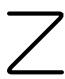
\includegraphics[keepaspectratio]{images/part001_3ab49149.jpg}}

\begin{enumerate}
\def\labelenumi{\arabic{enumi})}
\setcounter{enumi}{1}
\tightlist
\item
  Let \(\mathfrak{g} \subset \mathfrak{gl}(V)\) , \(\mathfrak{g}' \subset \mathfrak{gl}(V')\) be decomposable Lie algebras, \(\varphi\) an isomorphism from \(\mathfrak{g}\) to \(\mathfrak{g}'\) . Note that \(\varphi\) does not necessarily transform semi-simple (resp. nilpotent) elements of \(\mathfrak{g}\) to semi-simple (resp. nilpotent) elements of \(\mathfrak{g}'\) (Exerc. 2). However, this is the case if \(\mathfrak{g}\) is semi-simple (Chap. I, §6, no. 3, Th. 3).
\end{enumerate}

PROPOSITION 3. Let \(\mathfrak{a}\) be a decomposable Lie subalgebra of \(\mathfrak{gl}(\mathrm{V})\) and let \(\mathfrak{b}\) and \(\mathfrak{c}\) be vector subspaces of \(\mathfrak{gl}(\mathrm{V})\) such that \(\mathfrak{b} \subset \mathfrak{c}\) . Let \(\mathfrak{a}'\) be the set of \(x \in \mathfrak{a}\) such that \([x, \mathfrak{c}] \subset \mathfrak{b}\) . Then \(\mathfrak{a}'\) is decomposable.

Put \(\mathfrak{g} = \mathfrak{gl}(\mathrm{V})\) ; the subalgebra \(\mathfrak{h}'\) of \(\mathfrak{gl}(\mathfrak{g})\) consisting of the \(z \in \mathfrak{gl}(\mathfrak{g})\) such that \(z(\mathfrak{c}) \subset \mathfrak{b}\) is decomposable (Example 1). Let \(\pi : \mathfrak{g} \to \mathfrak{gl}(\mathfrak{g})\) be the adjoint representation of \(\mathfrak{g}\) . Prop. 2 (iv), applied to \(\pi\) , shows that \(\pi^{-1}(\mathfrak{h}')\) is decomposable. Hence so is \(\mathfrak{a}' = \mathfrak{a} \cap \pi^{-1}(\mathfrak{h}')\) .

COROLLARY 1. If \(\mathfrak{a}\) is a decomposable Lie subalgebra of \(\mathfrak{gl}(\mathrm{V})\) , and \(\mathfrak{n}\) a Lie subalgebra of \(\mathfrak{a}\) , the normalizer (resp. centralizer) of \(\mathfrak{n}\) in \(\mathfrak{a}\) is decomposable.

This follows from Prop. 3 by taking \(\mathfrak{c} = \mathfrak{n},\mathfrak{b} = \mathfrak{n}\) (resp. \(\mathfrak{c} = \mathfrak{n},\mathfrak{b} = \{0\}\) ).

COROLLARY 2. The Cartan subalgebras of a decomposable Lie subalgebra of \(\mathfrak{gl}(\mathrm{V})\) are decomposable.

This follows from Corollary 1.

Remark. We shall prove later (no. 5, Th. 2) a converse of Cor. 2.

\subsection{DECOMPOSABLE ENVELOPE}

The intersection of a family of decomposable Lie subalgebras of \(\mathfrak{gl}(V)\) is clearly decomposable. Consequently, if g is a Lie subalgebra of \(\mathfrak{gl}(V)\) , the set of decomposable Lie subalgebras of \(\mathfrak{gl}(V)\) containing g has a smallest element, called the decomposable envelope of g; in this paragraph, this envelope will be denoted by \(e(\mathfrak{g})\) .

PROPOSITION 4. Let \(\mathfrak{g}\) be a Lie subalgebra of \(\mathfrak{gl}(\mathrm{V})\) and \(\mathfrak{n}\) an ideal of \(\mathfrak{g}\) . Then \(\mathfrak{n}\) and \(e(\mathfrak{n})\) are ideals of \(e(\mathfrak{g})\) , and \([e(\mathfrak{g}), e(\mathfrak{n})] = [\mathfrak{g}, \mathfrak{n}]\) .

Let \(\mathfrak{g}_1\) be the set of \(x\in \mathfrak{gl}(\mathrm{V})\) such that \([x,\mathfrak{n}]\subset [\mathfrak{g},\mathfrak{n}]\) . This is a decomposable Lie subalgebra of \(\mathfrak{gl}(\mathrm{V})\) , containing \(\mathfrak{g}\) and hence \(e(\mathfrak{g})\) , cf.~no. 1, Prop. 3; in other words, \([e(\mathfrak{g}),\mathfrak{n}]\subset [\mathfrak{g},\mathfrak{n}]\) . Let \(\mathfrak{n}_1\) be the set of \(y\in \mathfrak{gl}(\mathrm{V})\) such that

\[
[ e (\mathfrak {g}), y ] \subset [ \mathfrak {g}, \mathfrak {n} ].
\]

This is a decomposable Lie subalgebra of \(\mathfrak{gl}(V)\) containing n by the preceding, and hence containing \(e(\mathfrak{n})\) ; in other words \([e(\mathfrak{g}), e(\mathfrak{n})] \subset [\mathfrak{g}, \mathfrak{n}]\) , so

\[
[ e (\mathfrak {g}), e (\mathfrak {n}) ] = [ \mathfrak {g}, \mathfrak {n} ].
\]

It follows that \([e(\mathfrak{g}),\mathfrak{n}]\subset [e(\mathfrak{g}),e(\mathfrak{n})]\subset \mathfrak{n}\) , so \(\mathfrak{n}\) and \(e(\mathfrak{n})\) are ideals of \(e(\mathfrak{g})\) .

COROLLARY 1. (i) \(\mathcal{D}^i\mathfrak{g} = \mathcal{D}^i e(\mathfrak{g})\) for \(i\geq 1\) , and \(\mathcal{C}^i\mathfrak{g} = \mathcal{C}^i e(\mathfrak{g})\) for \(i\geq 2\) .

\begin{enumerate}
\def\labelenumi{(\roman{enumi})}
\setcounter{enumi}{1}
\tightlist
\item
  If g is commutative (resp. nilpotent, resp. solvable), then \(e(\mathfrak{g})\) is commutative (resp. nilpotent, resp. solvable).
\end{enumerate}

Assertion (i) follows from Prop. 4 by induction on i and (ii) follows from (i).

COROLLARY 2. Let \(\mathfrak{r}\) be the radical of \(\mathfrak{g}\) . If \(\mathfrak{g}\) is decomposable, \(\mathfrak{r}\) is decomposable.

Indeed, \(e(\mathfrak{r})\) is a solvable ideal of \(\mathfrak{g}\) by Prop. 4 and Cor. 1, hence \(e(\mathfrak{r}) = \mathfrak{r}\) .

\subsection{DECOMPOSITIONS OF DECOMPOSABLE ALGEBRAS}

If g is a Lie subalgebra of \(\mathfrak{gl}(V)\) with radical r, the set of nilpotent elements of r is a nilpotent ideal of g, the largest nilpotency ideal of the identity representation of g (Chap. I, §5, no. 3, Cor. 6 of Th. 1). In this paragraph, we shall denote this ideal by \(\mathfrak{n}_{\mathrm{V}}(\mathfrak{g})\) . It contains the nilpotent radical \([g,g]\cap r\) of g (Chap. I, §5, no. 3, Th. 1).

PROPOSITION 5. Let g be a decomposable nilpotent Lie subalgebra of \(\mathfrak{gl}(V)\) . Let t be the set of semi-simple elements of g. Then t is a central subalgebra of g, and g is the product of t and \(\mathfrak{n}_{\mathrm{V}}(\mathfrak{g})\) as Lie algebras.

If \(x \in t\) , \(ad_{g}x\) is semi-simple and nilpotent, hence zero, so that x is central in g. Consequently, t is an ideal of g, and \(t \cap \mathfrak{n}_{\mathrm{V}}(\mathfrak{g}) = 0\) . Since g is decomposable, \(\mathfrak{g} = \mathfrak{t} + \mathfrak{n}_{\mathrm{V}}(\mathfrak{g})\) , hence the proposition.

PROPOSITION 6. Let g be a decomposable Lie subalgebra of \(\mathfrak{gl}(\mathrm{V})\) . Let T be the set of commutative subalgebras of g consisting of semi-simple elements, and \(T_{1}\) the set of maximal elements of T. Let H be the set of Cartan subalgebras of g.

\begin{enumerate}
\def\labelenumi{(\roman{enumi})}
\item
  For \(\mathfrak{h} \in \mathcal{H}\) , let \(\varphi(\mathfrak{h})\) be the set of semi-simple elements of \(\mathfrak{h}\) . Then \(\varphi(\mathfrak{h}) \in \mathcal{T}_1\) .
\item
  For \(\mathfrak{t} \in \mathcal{T}_1\) , let \(\psi(\mathfrak{t})\) be the commutant of \(\mathfrak{t}\) in \(\mathfrak{g}\) . Then \(\psi(\mathfrak{t}) \in \mathscr{H}\) .
\item
  The maps \(\varphi\) and \(\psi\) are inverse bijections from \(\mathcal{H}\) to \(\mathcal{T}_1\) and from \(\mathcal{T}_1\) to \(\mathcal{H}\) .
\item
  If \(k\) is algebraically closed, \(\mathrm{Aut}_e(\mathfrak{g})\) operates transitively on \(\mathcal{T}_1\) .
\end{enumerate}

Let \(\mathfrak{h} \in \mathcal{H}\) , and put \(\mathfrak{t} = \varphi(\mathfrak{h})\) . By Prop. 5 and Cor. 2 of Prop. 3, \(\mathfrak{t} \in \mathcal{T}\) and \(\mathfrak{h} = \mathfrak{t} \times \mathfrak{n}_{\mathrm{V}}(\mathfrak{h})\) . For any subalgebra \(\mathfrak{u}\) of \(\mathfrak{g}\) , we denote by \(\psi(\mathfrak{u})\) the commutant of \(\mathfrak{u}\) in \(\mathfrak{g}\) . Then \(\mathfrak{h} \subset \psi(\mathfrak{t})\) , and \(\psi(\mathfrak{t}) \subset \mathfrak{g}^0(\mathfrak{h})\) since the elements of \(\mathfrak{n}_{\mathrm{V}}(\mathfrak{h})\) are nilpotent, so \(\mathfrak{h} = \psi(\mathfrak{t})\) . If \(\mathfrak{t}' \in \mathcal{T}\) and \(\mathfrak{t} \subset \mathfrak{t}'\) , we have \(\mathfrak{t}' \subset \psi(\mathfrak{t}) = \mathfrak{h}\) so \(\mathfrak{t}' = \mathfrak{t}\) , and hence \(\mathfrak{t} \in \mathcal{T}_1\) .

Let \(\mathfrak{t} \in \mathcal{T}_1\) , and put \(\mathfrak{c} = \psi(\mathfrak{t})\) . Let \(\mathfrak{h}\) be a Cartan subalgebra of \(\mathfrak{c}\) . By §2, no. 3, Prop. 10, \(\mathfrak{h} \in \mathcal{H}\) and \(\mathfrak{t} \subset \mathfrak{h}\) . Put \(\mathfrak{t}_1 = \varphi(\mathfrak{h}) \in \mathcal{T}\) . Then \(\mathfrak{t} \subset \mathfrak{t}_1\) so \(\mathfrak{t} = \mathfrak{t}_1\) , and \(\mathfrak{h} = \psi(\mathfrak{t}_1) = \psi(\mathfrak{t}) = \mathfrak{c}\) by the preceding. Thus, \(\psi(\mathfrak{t}) \in \mathcal{H}\) , and \(\varphi(\psi(\mathfrak{t})) = \mathfrak{t}\) .

We have thus proved (i), (ii) and (iii). Assume that \(k\) is algebraically closed. Since \(\mathrm{Aut}_e(\mathfrak{g})\) operates transitively on \(\mathcal{H}(\S 3, \text{no. } 2, \text{Th. } 1)\) , \(\mathrm{Aut}_e(\mathfrak{g})\) operates transitively on \(\mathcal{T}_1\) .

COROLLARY 1. The Cartan subalgebras of \(\mathfrak{g}\) are the centralizers of the regular semi-simple elements of \(\mathfrak{g}\) .

If \(x \in \mathfrak{g}\) is regular, \(\mathfrak{g}^0(x)\) is a Cartan subalgebra of \(\mathfrak{g}\) (§2, no. 3, Th. 1 (i)); moreover, if \(x\) is semi-simple \(\mathfrak{g}^0(x)\) is the centralizer of \(x\) in \(\mathfrak{g}\) . Conversely, let \(\mathfrak{h}\) be a Cartan subalgebra of \(\mathfrak{g}\) . There exists \(\mathfrak{t} \in \mathcal{T}_1\) such that \(\mathfrak{h} = \psi(\mathfrak{t})\) . By §1, no. 2, Prop. 7, there exists \(x \in \mathfrak{t}\) such that \(\mathfrak{h} = \mathfrak{g}^0(x)\) ; since \(x \in \mathfrak{t}\) , \(\mathfrak{g}^0(x) = \mathfrak{g}_0(x)\) . By §3, no. 3, Th. 2 (ii), \(x\) is regular.

COROLLARY 2. Assume in addition that g is solvable. Then:

\begin{enumerate}
\def\labelenumi{(\roman{enumi})}
\item
  The subgroup of \(\operatorname{Aut}(\mathfrak{g})\) consisting of the \(e^{\mathrm{ad}x}, x \in \mathcal{C}^{\infty}\mathfrak{g}\) (cf.~§3, no. 4), operates transitively on \(\mathcal{T}_1\) .
\item
  If \(\mathfrak{t} \in \mathcal{T}_1\) , \(\mathfrak{g}\) is the semi-direct product of \(\mathfrak{t}\) and \(\mathfrak{n}_{\mathrm{V}}(\mathfrak{g})\) .
\end{enumerate}

Assertion (i) follows from the fact that the group of the \(e^{\mathrm{ad}x}\) , \(x \in \mathcal{C}^{\infty}\mathfrak{g}\) , operates transitively on \(\mathcal{H}(\S 3\) , no. 4, Th. 3).

We prove (ii). Let \(t \in T_{1}\) , and let \(\mathfrak{h} = \psi(t)\) be the corresponding Cartan subalgebra of g. In view of Prop. 5, \(\mathfrak{h} = \mathfrak{t} + \mathfrak{n}_{\mathrm{V}}(\mathfrak{h}) \subset \mathfrak{t} + \mathfrak{n}_{\mathrm{V}}(\mathfrak{g})\) . On the other hand, \(g = h + [g, g]\) (§2, no. 1, Cor. 3 of Prop. 4) and \([\mathfrak{g}, \mathfrak{g}] \subset \mathfrak{n}_{\mathrm{V}}(\mathfrak{g})\) , so \(\mathfrak{g} = \mathfrak{t} + \mathfrak{n}_{\mathrm{V}}(\mathfrak{g})\) . But it is clear that \(\mathfrak{t} \cap \mathfrak{n}_{\mathrm{V}}(\mathfrak{g}) = \{0\}\) . The algebra g is thus the semi-direct product of t and the ideal \(\mathfrak{n}_{\mathrm{V}}(\mathfrak{g})\) .

PROPOSITION 7. Let \(\mathfrak{g}\) be a decomposable Lie subalgebra of \(\mathfrak{gl}(\mathrm{V})\) .

\begin{enumerate}
\def\labelenumi{(\roman{enumi})}
\item
  There exists a Lie subalgebra \(\mathfrak{m}\) of \(\mathfrak{g}\) , reductive in \(\mathfrak{gl}(\mathrm{V})\) , such that \(\mathfrak{g}\) is the semi-direct product of \(\mathfrak{m}\) and \(\mathfrak{n}_{\mathrm{V}}(\mathfrak{g})\) .
\item
  Any two Lie subalgebras of \(\mathfrak{g}\) with the properties in (i) are conjugate under \(\mathrm{Aut}_e(\mathfrak{g})\) .
\end{enumerate}

The radical r of g is decomposable (no. 2, Cor. 2 of Prop. 4). By Cor. 2 of Prop. 6, there exists a commutative subalgebra t of r, consisting of semi-simple elements, such that \(\mathfrak{r} = \mathfrak{t} \oplus \mathfrak{n}_{\mathrm{V}}(\mathfrak{r})\) . Since \(ad_{g}t\) consists of semi-simple elements, g is the direct sum of \([t, g]\) and the centralizer z of t (Chap. I, §3, no. 5, Prop. 6). Since \([t, g] \subset r\) , \(g = z + r\) . Consequently, if s is a Levi subalgebra of z (Chap. I, §6, no. 8), \(g = s + r\) , so s is a Levi subalgebra of g. Put \(m = s \oplus t\) . Since \([s, t] = \{0\}\) , m is a Lie subalgebra of g, reductive in \(\mathfrak{gl}(V)\) by Chap. I, §6, no. 5, Th. 4. Moreover,

\[
\mathfrak {g} = \mathfrak {s} \oplus \mathfrak {r} = \mathfrak {s} \oplus \mathfrak {t} \oplus \mathfrak {n} _ {\mathrm{V}} (\mathfrak {r}) = \mathfrak {s} \oplus \mathfrak {t} \oplus \mathfrak {n} _ {\mathrm{V}} (\mathfrak {g}) = \mathfrak {m} \oplus \mathfrak {n} _ {\mathrm{V}} (\mathfrak {g})
\]

since \(\mathfrak{n}_{\mathrm{V}}(\mathfrak{g}) = \mathfrak{n}_{\mathrm{V}}(\mathfrak{r})\) . Hence (i).

Now let \(\mathfrak{m}'\) be a Lie subalgebra of \(\mathfrak{g}\) complementary to \(\mathfrak{n}_{\mathrm{V}}(\mathfrak{g})\) and reductive in \(\mathfrak{gl}(\mathrm{V})\) . We show that \(\mathfrak{m}'\) is conjugate to \(\mathfrak{m}\) under \(\operatorname{Aut}_e(\mathfrak{g})\) . We have \(\mathfrak{m}' = \mathfrak{s}' \oplus \mathfrak{t}'\) , where \(\mathfrak{s}' = [\mathfrak{m}', \mathfrak{m}']\) is semi-simple and the centre \(\mathfrak{t}'\) of \(\mathfrak{m}'\) consists of semi-simple elements. Then \(\mathfrak{r} = \mathfrak{t} \oplus \mathfrak{n}_{\mathrm{V}}(\mathfrak{g}) = \mathfrak{t}' \oplus \mathfrak{n}_{\mathrm{V}}(\mathfrak{g})\) . In view of Cor. 2 of Prop. 6, we are reduced to the case \(\mathfrak{t} = \mathfrak{t}'\) . Then \(\mathfrak{s}' \subset \mathfrak{z}\) ; since \(\dim \mathfrak{s}' = \dim \mathfrak{s}\) , \(\mathfrak{s}'\) is a Levi subalgebra of \(\mathfrak{z}\) . By Chap. I, §6, no. 8, Th. 5, there exists \(x \in \mathfrak{n}_{\mathrm{V}}(\mathfrak{z})\) such that \(e^{\operatorname{ad} x}(\mathfrak{s}) = \mathfrak{s}'\) ; since \(x\) commutes with \(\mathfrak{t}\) , we also have \(e^{\operatorname{ad} x}(\mathfrak{t}) = \mathfrak{t}\) .

\subsection{LINEAR LIE ALGEBRAS OF NILPOTENT ENDOMORPHISMS}

Lemma 1. Let \(\mathfrak{n}\) be a Lie subalgebra of \(\mathfrak{gl}(\mathrm{V})\) consisting of nilpotent endomorphisms, and \(\mathrm{N}\) the subgroup \(\exp \mathfrak{n}\) of \(\mathbf{GL}(\mathrm{V})\) (§3, no. 1, Lemma 1).

\begin{enumerate}
\def\labelenumi{(\roman{enumi})}
\item
  Let \(\rho\) be a finite dimensional linear representation of \(\mathfrak{n}\) on W, such that the elements of \(\rho(\mathfrak{n})\) are nilpotent, W' a vector subspace of W stable under \(\rho\) , \(\rho_1\) and \(\rho_2\) the subrepresentation and quotient representation of \(\rho\) defined by W', \(\pi, \pi_1, \pi_2\) the representations of N compatible with \(\rho, \rho_1, \rho_2\) (§3, no. 1). Then \(\pi_1, \pi_2\) are the subrepresentation and quotient representation of \(\pi\) defined by W'.
\item
  Let \(\rho_1, \rho_2\) be finite dimensional linear representations of \(\mathfrak{n}\) such that the elements of \(\rho_1(\mathfrak{n})\) and \(\rho_2(\mathfrak{n})\) are nilpotent, and \(\pi_1, \pi_2\) the representations of N compatible with \(\rho_1, \rho_2\) . Then \(\pi_1 \otimes \pi_2\) is the representation of N compatible with \(\rho_1 \otimes \rho_2\) .
\item
  Let \(\rho_{1},\rho_{2}\) be finite dimensional linear representations of \(\mathfrak{n}\) on vector spaces \(V_{1},V_{2}\) , such that the elements of \(\rho_1(\mathfrak{n})\) and \(\rho_{2}(\mathfrak{n})\) are nilpotent, \(\rho\) the representation of \(\mathfrak{n}\) on \(\mathrm{Hom}(V_1,V_2)\) determined by \(\rho_{1},\rho_{2}\) . Let \(\pi_1,\pi_2\) be the representations of N compatible with \(\rho_{1},\rho_{2}\) , and \(\pi\) the representation of N on \(\mathrm{Hom}(\mathrm{V}_1,\mathrm{V}_2)\) determined by \(\pi_1,\pi_2\) . Then \(\pi\) is the representation of N compatible with \(\rho\) .
\end{enumerate}

Assertion (i) is clear. Let \(\rho_1, \rho_2, \pi_1, \pi_2\) be as in (ii). If \(x \in \mathfrak{n}\) , we have, since \(\rho_1(x) \otimes 1\) and \(1 \otimes \rho_2(x)\) commute,

\[
\begin{array}{l} \exp (\rho_ {1} (x) \otimes 1 + 1 \otimes \rho_ {2} (x)) = \exp (\rho_ {1} (x) \otimes 1). \exp (1 \otimes \rho_ {2} (x)) \\ \qquad = (\exp \rho_ {1} (x)) \otimes 1. 1 \otimes (\exp \rho_ {2} (x)) \\ \qquad = (\exp \rho_ {1} (x)) \otimes (\exp \rho_ {2} (x)) \\ \qquad = \pi_ {1} (\exp x) \otimes \pi_ {2} (\exp x) \\ \qquad = (\pi_ {1} \otimes \pi_ {2}) (\exp x), \end{array}
\]

hence (ii). Let \(\rho_1, \rho_2, \rho, \pi_1, \pi_2, \pi, V_1, V_2\) be as in (iii). If \(v_1 \in \mathrm{End}V_1\) and \(v_2 \in \mathrm{End}V_2\) , denote by \(R_{v_1}\) and \(L_{v_2}\) the maps \(u \mapsto uv_1\) and \(u \mapsto v_2u\) from \(\mathrm{Hom}(V_1, V_2)\) to itself; these maps commute and \(\rho(x)u = (L_{\rho_2(x)} - R_{\rho_1(x)})u\) , so

\[
\begin{array}{r l} & {\exp \rho (x). u = \exp \mathrm{L} _ {\rho_ {2} (x)}. \exp \mathrm{R} _ {- \rho_ {1} (x)}. u} \\ & {\qquad = \mathrm{L} _ {\exp \rho_ {2} (x)}. \mathrm{R} _ {\exp (- \rho_ {1} (x))}. u} \\ & {\qquad = \mathrm{L} _ {\pi_ {2} (\exp x)}. \mathrm{R} _ {\pi_ {1} (\exp (- x))}. u} \\ & {\qquad = \pi (\exp x). u,} \end{array}
\]

hence (iii).

Lemma 2 \(^{2}\) . (i) Let W be a vector subspace of V of dimension d, D the line \(\bigwedge^{d}\) W \(\subset \bigwedge^{d}\) V, \(\theta\) the canonical representation of \(\mathfrak{gl}(V)\) on \(\bigwedge V\) (Chap. III, App.). Let \(x \in \mathfrak{gl}(V)\) . Then \(x(W) \subset W\) if and only if \(\theta(x)(D) \subset D\) .

\begin{enumerate}
\def\labelenumi{(\roman{enumi})}
\setcounter{enumi}{1}
\tightlist
\item
  Let \((e_{1},\ldots,e_{n})\) be the canonical basis of \(k^{n}\) , \(\theta\) the canonical representation of \(\mathfrak{gl}(n,k)\) on \(\bigwedge(k^{n})\) , and \(x\in\mathfrak{gl}(n,k)\) . Then \(x\in\mathfrak{n}(n,k)\) if and only if
\end{enumerate}

\[
\theta (x) (e _ {n - d + 1} \wedge \dots \wedge e _ {n}) = 0
\]

for \(1 \leq d \leq n\) .

\footnotetext[2]{In this lemma, \(k\) can be an arbitrary (commutative) field.}

\begin{enumerate}
\def\labelenumi{(\roman{enumi})}
\tightlist
\item
  If \(x(\mathrm{W}) \subset \mathrm{W}\) , it is clear that \(\theta(x)\mathrm{D} \subset \mathrm{D}\) . Conversely, assume that \(\theta(x)\mathrm{D} \subset \mathrm{D}\) . Let \(u\) be a non-zero element of \(\mathrm{D}\) and let \(y \in \mathrm{W}\) . Then \(y \wedge u = 0\) . Since \(\theta(x)\) is a derivation of \(\bigwedge \mathrm{V}\) , this implies
\end{enumerate}

\[
\theta (x) y \wedge u + y \wedge \theta (x) u = 0.
\]

Now \(\theta(x)u\in ku\) , so \(y\wedge\theta(x)u=0\) and consequently \(\theta(x)y\wedge u=0\) . By Algebra, Chap. III, §7, no. 9, Prop. 13, this implies that \(\theta(x)y\in W\) , i.e.~\(x(y)\in W\) , which proves that \(x(W)\subset W\) .

\begin{enumerate}
\def\labelenumi{(\roman{enumi})}
\setcounter{enumi}{1}
\tightlist
\item
  The condition stated in (ii) is clearly necessary for \(x \in \mathfrak{n}(n, k)\) . Assume that it is satisfied. By (i), \(x\) leaves
\end{enumerate}

\[
k e _ {n - d + 1} + \dots + k e _ {n}
\]

stable, and since this holds for \(d = 1, \ldots, n\) , \(x\) is lower triangular. Put

\[
x = (x _ {i j}) _ {1 \leq i, j \leq n}.
\]

We have \(0 = x(e_n) = x_{nn}e_n\) , so \(x_{nn} = 0\) . Let \(i < n\) , and assume that we have proved that \(x_{jj} = 0\) for \(j > i\) . Then

\[
0 = \theta (x) \left(e _ {i} \wedge e _ {i + 1} \wedge \dots \wedge e _ {n}\right) = x _ {i i} \left(e _ {i} \wedge e _ {i + 1} \wedge \dots \wedge e _ {n}\right),
\]

so \(x_{ii} = 0\) . Thus, \(x \in \mathfrak{n}(n,k)\) .

PROPOSITION 8. Let \(\mathfrak{n}\) be a Lie subalgebra of \(\mathfrak{gl}(\mathrm{V})\) consisting of nilpotent elements, \(\mathfrak{q}\) the normalizer of \(\mathfrak{n}\) in \(\mathfrak{gl}(\mathrm{V})\) . There exists a finite dimensional vector space E, a representation \(\rho\) of \(\mathfrak{gl}(\mathrm{V})\) on E, and a vector subspace F of E, satisfying the following conditions:

\begin{enumerate}
\def\labelenumi{(\roman{enumi})}
\item
  the image under \(\rho\) of a homothety of \(V\) is diagonalizable;
\item
  F is stable under \(\rho(\mathfrak{q})\) ;
\item
  \(\mathfrak{n}\) is the set of \(x\in \mathfrak{gl}(\mathrm{V})\) such that \(\rho (x)(\mathrm{F}) = 0\)
\end{enumerate}

Let \(n = \dim V\) . By Engel's theorem, \(V\) can be identified with \(k^n\) in such a way that \(\mathfrak{n} \subset \mathfrak{n}(n,k)\) . Let \(P\) be the algebra of polynomial functions on \(\mathfrak{gl}(n,k)\) . For \(i = 0,1,\ldots\) , let \(P_i\) be the set of elements of \(P\) homogeneous of degree \(i\) . Let \(N = \exp \mathfrak{n}\) , which is a subgroup of the strictly lower triangular group \(T\) . Let \(J\) be the set of elements of \(P\) that are zero on \(N\) ; this is an ideal in \(P\) . Let \(N_J\) be the set of \(x \in \mathfrak{gl}(n,k)\) such that \(p(x) = 0\) for all \(p \in J\) . Then \(N \subset N_J\) . Conversely, let \(x \in N_J\) . Denote by \(p_{ij}\) the polynomial functions giving the entries of an element of \(\mathfrak{gl}(n,k)\) . The ideal \(J\) contains the \(p_{ij}\) (for \(i < j\) ) and the \(p_{ii} - 1\) ; hence \(x \in T\) . On the other hand, if \(u\) is a linear form on \(\mathfrak{gl}(n,k)\) which is zero on \(\mathfrak{n}\) , there exists \(p_u \in P\) such that \(p_u(z) = u(\log z)\) for all \(z \in T\) ( \(\S 3\) , no. 1, Lemma 1 (i)); we have \(p_u \in J\) , so \(u(\log x) = 0\) . It follows that \(\log x\) belongs to \(\mathfrak{n}\) , so \(x \in N\) , proving that \(N = N_J\) .

For all \(p \in P\) and \(g \in \mathbf{GL}_{n}(k)\) , let \(\lambda(g)p\) be the function \(x \mapsto p(g^{-1}x)\) on \(\mathfrak{gl}(n,k)\) ; then \(\lambda(g)p \in \mathrm{P}\) , \(\lambda(g)\) is an automorphism of the algebra P, and \(\lambda\) is a representation of \(\mathbf{GL}_{n}(k)\) on P which leaves each \(P_{i}\) stable. We show that

\[
\mathrm{N} = \{x \in \mathbf {G L} _ {n} (k) \mid \lambda (x) \mathrm{J} = \mathrm{J} \}.\tag{1}
\]

If \(x \in \mathrm{N}, p \in \mathrm{J}, y \in \mathrm{N}\) , then \((\lambda(x)p)(y) = p(x^{-1}y) = 0\) since \(x^{-1}y \in \mathrm{N}\) ; thus \(\lambda(x)p \in \mathrm{J}\) , so \(\lambda(x)\mathrm{J} = \mathrm{J}\) . Let \(x \in \mathbf{GL}_n(k)\) be such that \(\lambda(x)\mathrm{J} = \mathrm{J}\) ; let \(p \in \mathrm{J}\) ; then \(p(x^{-1}) = (\lambda(x)p)(e) = 0\) , so \(x^{-1} \in \mathrm{N}_{\mathrm{J}} = \mathrm{N}\) and \(x \in \mathrm{N}\) . This proves (i).

The ideal J is of finite type (Commutative Algebra, Chap. III, §2, no. 10, Cor. 2 of Th. 2). Hence, there exists an integer q such that, if \(W = P_{0} + P_{1} + \cdots + P_{q}\) , then \(J \cap W\) generates J as an ideal. Denote by \(\lambda_{j}\) (resp. \(\lambda'\) ) the subrepresentation of \(\lambda\) defined by \(P_{J}\) (resp. by W). By (1),

\[
\mathrm{N} = \{x \in \mathbf {G L} _ {n} (k) \mid \lambda^ {\prime} (x) (\mathrm{J} \cap \mathrm{W}) = \mathrm{J} \cap \mathrm{W} \}.\tag{2}
\]

We show that, for all \(j\) , there exists a representation \(\sigma_{j}\) of the Lie algebra \(\mathfrak{gl}(n,k)\) on \(\mathrm{P}_j\) such that:

\[
\sigma_ {j} | \mathfrak {n} (n, k) \text {   is   compatible   } (\S 3, \text {   no.   } 1) \text {   with   } \lambda_ {j} | T.\tag{3}
\]

\[
\text { For   all } x \in k. 1 _ {n}, \sigma_ {j} (x) \text { is   a   homothety. }\tag{4}
\]

Since \(\lambda_{j}\) is the jth symmetric power of \(\lambda_{1}\) , it suffices to prove the existence of \(\sigma_{1}\) , cf.~Lemma 1. Now \(\lambda_{1}\) is the contragredient representation of the representation \(\gamma\) of \(\mathbf{GL}_{n}(k)\) on \(\mathfrak{gl}(n,k)\) given by

\[
\gamma (x) y = x y, \quad x \in \mathbf {G L} _ {n} (k), \quad y \in \mathfrak {g l} (n, k).
\]

Let \(c\) be the representation of the Lie algebra \(\mathfrak{gl}(n,k)\) on \(\mathfrak{gl}(n,k)\) given by

\[
c (x) y = x y, \quad x, y \in \mathfrak {g l} (n, k).
\]

It is immediate that \(c|\mathfrak{n}(n,k)\) and \(\gamma|T\) are compatible, and that \(c(x)\) is a homothety for all \(x \in k.1_{n}\) . Thus, it suffices to take for \(\sigma_{1}\) the dual representation of c (Chap. I, §3, no. 3).

Now let \(\sigma'\) be the representation of \(\mathfrak{gl}(n,k)\) on W given by the direct sum of the \(\sigma_j\) , \(0 \leq j \leq q\) . In view of (2) and the relations

\[
\lambda^ {\prime} (\exp (x)) = \exp (\sigma^ {\prime} (x)) \text { and } \sigma^ {\prime} (\log (y)) = \log (\lambda^ {\prime} (y)), x \in \mathfrak {n} (n, k), y \in \mathrm{T},
\]

we have

\[
\mathfrak {n} = \{x \in \mathfrak {n} (n, k) \mid \sigma^ {\prime} (x) (\mathrm{J} \cap \mathrm{W}) \subset \mathrm{J} \cap \mathrm{W} \}.\tag{5}
\]

Let \(d = \dim(\mathrm{J} \cap \mathrm{W})\) , and let \(\tau = \bigwedge^{d} \sigma'\) . Let \(\mathrm{D} = \bigwedge^{d} (\mathrm{J} \cap \mathrm{W})\) . By (5) and Lemma 2 (i),

\[
\mathfrak {n} = \{x \in \mathfrak {n} (n, k) \mid \tau (x) (\mathrm{D}) \subset \mathrm{D} \}.\tag{6}
\]

But \(\tau (\mathfrak{n}(n,k))\) consists of nilpotent endomorphisms, so (6) can also be written

\[
\mathfrak {n} = \{x \in \mathfrak {n} (n, k) \mid \tau (x) (\mathrm{D}) = 0 \}.\tag{7}
\]

Now let \(E = \bigwedge^{d} W \oplus \bigwedge^{1} V \oplus \bigwedge^{2} V \oplus \cdots \oplus \bigwedge^{n} V\) ; let \(\rho\) be the direct sum of \(\tau\) and the canonical representations of \(\mathfrak{gl}(n, k)\) on \(\bigwedge^{1} V, \ldots, \bigwedge^{n} V\) . Let \(E_{0} \subset E\) be the sum of \(D = \bigwedge^{d} (J \cap W)\) and the lines generated by \(e_{n-j+1} \wedge \cdots \wedge e_{n}\) for \(j = 1, \ldots, n\) . By (7) and Lemma 2 (ii),

\[
\mathfrak {n} = \{x \in \mathfrak {g l} (\mathrm{V}) \mid \rho (x) (\mathrm{E} _ {0}) = 0 \}.\tag{8}
\]

It is immediate that, if \(x \in k.1_{n}\) , \(\rho(x)\) is diagonalizable. Finally, if F is the set of elements of E annihilated by \(\rho(\mathfrak{n})\) , F is stable under \(\rho(\mathfrak{q})\) (Chap. I, §3, no. 5, Prop. 5), and by (8),

\[
\mathfrak {n} = \{x \in \mathfrak {g l} (\mathrm{V}) \mid \rho (x) (\mathrm{F}) = 0 \}.\tag{9}
\]

\subsection{CHARACTERIZATIONS OF DECOMPOSABLE LIE ALGEBRAS}

Every decomposable Lie algebra is generated as a vector space (and a fortiori as a Lie algebra) by the set of its elements that are either semi-simple or nilpotent. Conversely:

THEOREM 1. Let g be a Lie subalgebra of \(\mathfrak{gl}(V)\) and let X be a subset of g generating g as a Lie algebra over k. If every element of X is either semi-simple or nilpotent, g is decomposable.

\begin{enumerate}
\def\labelenumi{\alph{enumi})}
\tightlist
\item
  \(\mathfrak{g}\) is commutative.
\end{enumerate}

The semi-simple (resp. nilpotent) elements of g form a vector subspace \(g_{s}\) (resp. \(g_{n}\) ). The assumption is equivalent to \(g = g_{s} \oplus g_{n}\) , hence the fact that g is decomposable.

\begin{enumerate}
\def\labelenumi{\alph{enumi})}
\setcounter{enumi}{1}
\tightlist
\item
  \(\mathfrak{g}\) is reductive.
\end{enumerate}

Then \(\mathfrak{g} = \mathfrak{g}' \times \mathfrak{c}\) with \(\mathfrak{g}'\) semi-simple and \(\mathfrak{c}\) commutative. By Prop. 2, \(\mathfrak{g}'\) is decomposable. Let \(x = a + b \in \mathfrak{g}\) with \(a \in \mathfrak{g}'\) , \(b \in \mathfrak{c}\) . Let \(a_s, a_n, b_s, b_n\) be the semi-simple and nilpotent components of \(a, b\) . Since \(a_s, a_n, b_s, b_n\) mutually commute, the semi-simple and nilpotent components of \(x\) are \(a_s + b_s, a_n + b_n\) . Now \(a_s, a_n \in \mathfrak{g}'\) . If \(x\) is semi-simple, \(x = a_s + b_s\) ; since \(a_s \in \mathfrak{g}'\) , we have \(b_s \in \mathfrak{g}\) , so \(b_s \in \mathfrak{c}\) since \(b_s\) commutes with \(\mathfrak{g}\) ; consequently, \(a = a_s\) and \(b = b_s\) . Similarly, if \(x\) is nilpotent, \(a = a_n\) and \(b = b_n\) . It follows that the projections on \(\mathfrak{c}\) of the elements of X are either semi-simple or nilpotent; by \(a)\) , this implies that \(\mathfrak{c}\) is decomposable. Retaining the preceding notation, but without the assumption on \(x\) , we now have \(b_s, b_n \in \mathfrak{c}\) , so \(a_s + b_s, a_n + b_n \in \mathfrak{g}\) , which proves the theorem in this case.

\begin{enumerate}
\def\labelenumi{\alph{enumi})}
\setcounter{enumi}{2}
\tightlist
\item
  General case.
\end{enumerate}

We assume that the theorem is proved for Lie algebras of dimension \(< \dim \mathfrak{g}\) and prove it for \(\mathfrak{g}\) .

Let \(\mathfrak{n}\) be the largest ideal of nilpotency of the identity representation of \(\mathfrak{g}\) . If \(\mathfrak{n} = 0\) , \(\mathfrak{g}\) has an injective semi-simple representation, and so is reductive. Assume that \(\mathfrak{n} \neq 0\) . Let \(\mathfrak{p}\) be the normalizer of \(\mathfrak{n}\) in \(\mathfrak{gl}(\mathrm{V})\) . There exist E, \(\rho, \mathrm{F}\) satisfying the conditions of Prop. 8. Since \(\mathfrak{g} \subset \mathfrak{p}\) , \(\rho(\mathfrak{g})\) leaves F stable; let \(\rho_0\) be the representation \(u \mapsto \rho(u)|\mathrm{F}\) of \(\mathfrak{g}\) on F; we have \(\mathfrak{n} = \mathrm{Ker}\rho_0\) . The image under \(\rho\) of every semi-simple (resp. nilpotent) element of \(\mathfrak{gl}(\mathrm{V})\) is semi-simple (resp. nilpotent) (Prop. 2). The algebra \(\rho_0(\mathfrak{g})\) is thus generated by its semi-simple elements and its nilpotent elements. By the induction hypothesis, \(\rho_0(\mathfrak{g})\) is decomposable.

Let \(x \in \mathfrak{g}\) , and let \(x_s, x_n\) be its semi-simple and nilpotent components. By Prop. 2, the semi-simple and nilpotent components of \(\rho(x)\) are \(\rho(x_s), \rho(x_n)\) . Since \(\rho_0(\mathfrak{g})\) is decomposable, there exist \(y, z \in \mathfrak{g}\) such that

\[
\rho_ {0} (y) = \rho (x _ {s}) | \mathrm{F}, \rho_ {0} (z) = \rho (x _ {n}) | \mathrm{F}.
\]

Then \(x_{s}\in y + \mathfrak{n},x_{n}\in z + \mathfrak{n}\) , so \(x_{s},x_{n}\in \mathfrak{g}\)

Q.E.D.

COROLLARY 1. Every subalgebra of \(\mathfrak{gl}(\mathrm{V})\) generated by its decomposable subalgebras is decomposable.

This is clear.

COROLLARY 2. Let \(\mathfrak{g}\) be a Lie subalgebra of \(\mathfrak{gl}(\mathrm{V})\) . Then \([\mathfrak{g},\mathfrak{g}]\) is decomposable.

Let \(\mathfrak{r}\) be the radical of \(\mathfrak{g}\) , \(\mathfrak{s}\) a Levi subalgebra of \(\mathfrak{g}\) (Chap. I, §6, no. 8). Then

\[
[ \mathfrak {g}, \mathfrak {g} ] = [ \mathfrak {s}, \mathfrak {s} ] + [ \mathfrak {s}, \mathfrak {r} ] + [ \mathfrak {r}, \mathfrak {r} ] = \mathfrak {s} + [ \mathfrak {g}, \mathfrak {r} ].
\]

The algebra \([g,r]\) is decomposable since all of its elements are nilpotent (Chap. I, §5, no. 3). On the other hand, s is decomposable (Prop. 2). It follows that \([g,g]\) is decomposable (Cor. 1).

COROLLARY 3. Let \(\mathfrak{g}\) be a Lie subalgebra of \(\mathfrak{gl}(\mathrm{V})\) , and let \(\mathrm{X}\) be a subset of \(\mathfrak{g}\) generating \(\mathfrak{g}\) (as a Lie algebra over \(k\) ).

\begin{enumerate}
\def\labelenumi{(\roman{enumi})}
\item
  The decomposable envelope \(e(\mathfrak{g})\) of \(\mathfrak{g}\) is generated by the semi-simple and nilpotent components of the elements of \(X\) .
\item
  If \(k'\) is an extension of \(k\) , \(e(\mathfrak{g} \otimes_k k') = e(\mathfrak{g}) \otimes_k k'\) ; and \(\mathfrak{g}\) is decomposable if and only if \(\mathfrak{g} \otimes_k k'\) is decomposable.
\end{enumerate}

Let \(\tilde{\mathfrak{g}}\) be the subalgebra of \(\mathfrak{gl}(\mathrm{V})\) generated by the semi-simple and nilpotent components of the elements of X. Then \(\mathfrak{g} \subset \tilde{\mathfrak{g}} \subset e(\mathfrak{g})\) ; by Th. 1, \(\tilde{\mathfrak{g}}\) is decomposable, so \(\tilde{\mathfrak{g}} = e(\mathfrak{g})\) , which proves (i). Assertion (ii) follows, since X generates the \(k'\) -algebra \(\mathfrak{g} \otimes_k k'\) .

COROLLARY 4. Let g be a decomposable Lie subalgebra of \(\mathfrak{gl}(\mathrm{V})\) . Let T be the set of commutative subalgebras of g consisting of semi-simple elements (cf.~Prop. 6). The maximal elements of T all have the same dimension.

Let \(k'\) be an algebraically closed extension of \(k\) and \(V' = V \otimes_k k', \mathfrak{g}' = \mathfrak{g} \otimes_k k'\) . Let \(t_1, t_2\) be maximal elements of \(\mathcal{T}\) , \(t_i' = t_i \otimes_k k'\) , \(\mathfrak{h}_i\) the commutant of \(t_i\) in \(\mathfrak{g}\) , \(\mathfrak{h}_i' = \mathfrak{h}_i \otimes_k k'\) . Then \(\mathfrak{h}_i\) is a Cartan subalgebra of \(\mathfrak{g}\) (Prop. 6) so \(\mathfrak{h}_i'\) is a Cartan subalgebra of \(\mathfrak{g}'\) . Then \(\mathfrak{h}_i = t_i \times \mathfrak{n}_V(\mathfrak{h}_i)\) , hence \(\mathfrak{h}_i' = t_i' \times \mathfrak{n}_{V'}(\mathfrak{h}_i')\) , so that \(t_i'\) is the set of semi-simple elements of \(\mathfrak{h}_i'\) . Since \(\mathfrak{g}'\) is decomposable (Cor. 3), \(t_1'\) and \(t_2'\) are conjugate under \(\text{Aut}_e(\mathfrak{g}')\) (Prop. 6), so \(\dim t_1 = \dim t_2\) .

THEOREM 2. Let \(\mathfrak{g}\) be a Lie subalgebra of \(\mathfrak{gl}(\mathrm{V})\) . The following conditions are equivalent:

\begin{enumerate}
\def\labelenumi{(\roman{enumi})}
\item
  \(\mathfrak{g}\) is decomposable;
\item
  every Cartan subalgebra of \(\mathfrak{g}\) is decomposable;
\item
  \(\mathfrak{g}\) has a decomposable Cartan subalgebra;
\item
  the radical of \(\mathfrak{g}\) is decomposable.
\item
  \(\Longrightarrow\) (ii): This follows from Cor. 2 of Prop. 3.
\item
  \(\Longrightarrow\) (i): This follows from Cor. 1 of Th. 1, since \(\mathfrak{g}\) is generated by its Cartan subalgebras (§2, no. 3, Cor. 3 of Th. 1).
\item
  \(\Longrightarrow\) (iii): This is clear.
\item
  \(\Longrightarrow\) (ii): By Cor. 3 of Th. 1, we can assume that k is algebraically closed. The Cartan subalgebras of g are then conjugate under the elementary automorphisms of g (§3, no. 2, Th. 1); in view of Remark 1 of §3, no. 1, it follows that, if one of these is decomposable, they all are.
\item
  \(\Longrightarrow\) (iv): This follows from Cor. 2 of Prop. 4.
\item
  \(\Longrightarrow\) (i): Assume that the radical r of g is decomposable. Let s be a Levi subalgebra of g; it is decomposable (Prop. 2). Hence \(g = s + r\) is decomposable (Cor. 1 of Th. 1).
\end{enumerate}

\appendixsection{POLYNOMIAL MAPS AND ZARISKI TOPOLOGY}

In this appendix, \(k\) is assumed to be infinite.

\appendixitem{ZARISKI TOPOLOGY}

Let V be a finite dimensional vector space. We denote by \(A_{V}\) the algebra of polynomial functions on V with values in k (Algebra, Chap. IV, §5, no. 10, Def. 4). This is a graded algebra; its component of degree 1 is the dual \(V^{*}\) of V, and the injection of \(V^{*}\) into \(A_{V}\) extends to an isomorphism from the symmetric algebra \(\mathbf{S}(V^{*})\) to \(A_{V}\) (Algebra, Chap. IV, §5, no. 11, Remark 2).

If \((e_{1},\ldots,e_{n})\) is a basis of V, and \((\mathrm{X}_{1},\ldots,\mathrm{X}_{n})\) a sequence of indeterminates, the map from \(k[\mathrm{X}_{1},\ldots,\mathrm{X}_{n}]\) to \(A_{V}\) that takes any element f of \(k[\mathrm{X}_{1},\ldots,\mathrm{X}_{n}]\) to the function

\[
\sum_ {i = 1} ^ {n} \lambda_ {i} e _ {i} \mapsto f (\lambda_ {1}, \ldots , \lambda_ {n})
\]

is an isomorphism of algebras (Algebra, Chap. IV, §5, no. 10, Cor. of Prop. 19).

PROPOSITION 1. Let H be the set of algebra homomorphisms from \(A_{V}\) to k. For any \(x \in V\) , let \(h_{x}\) be the homomorphism \(f \mapsto f(x)\) from \(A_{V}\) to k. Then, the map \(x \mapsto h_{x}\) is a bijection from V to H.

Indeed, let \(\mathrm{H}'\) be the set of algebra homomorphisms from \(k[\mathrm{X}_1,\ldots ,\mathrm{X}_n]\) to \(k\) . The map \(\chi \mapsto (\chi (\mathrm{X}_1),\dots ,\chi (\mathrm{X}_n))\) is clearly a bijection from \(\mathrm{H}'\) to \(k^n\) .

COROLLARY. For any \(x \in V\) , let \(\mathfrak{m}_{x} = \operatorname{Ker}(h_{x})\) . Then the map \(x \mapsto \mathfrak{m}_{x}\) is a bijection from V to the set of ideals m of \(A_{V}\) such that \(A_{V}/m = k\) .

A subset \(\mathrm{F}\) of \(\mathrm{V}\) is said to be closed if there exists a family \((f_i)_{i\in \mathrm{I}}\) of elements of \(\mathrm{A_V}\) such that

\[
x \in \mathrm{F} \Longleftrightarrow x \in \mathrm{V} \text {   and   } f _ {i} (x) = 0 \text {   for   all   } i \in \mathrm{I}.
\]

It is clear that \(\varnothing\) and V are closed, and that any intersection of closed sets is closed. If F is defined by the vanishing of the \(f_{i}\) and \(\mathrm{F}'\) by that of the \(f_j'\) , \(\mathrm{F} \cup \mathrm{F}'\) is defined by the vanishing of the \(f_{i}f_{j}'\) , and hence is closed. Thus, there exists a topology on V such that the closed sets for this topology are exactly the closed sets in the above sense. This topology is called the Zariski topology on V. For any \(f \in \mathrm{A_V}\) , we denote by \(\mathrm{V}_f\) the set of \(x \in \mathrm{V}\) such that \(f(x) \neq 0\) ; this is an open subset of V. It is clear that the \(\mathrm{V}_f\) form a base of the Zariski topology. (If \(k\) is a topological field, the canonical topology of V is finer than the Zariski topology.)

The map \(x \mapsto m_{x}\) of the Cor. of Prop. 1 can be considered as a map \(\varepsilon\) from V to the prime spectrum \(\operatorname{Spec}(A_{\mathrm{V}})\) of \(A_{V}\) (Commutative Algebra, Chap. II, §4, no. 3, Def. 4). It is immediate that the Zariski topology is the inverse image under \(\varepsilon\) of the topology of \(\operatorname{Spec}(A_{\mathrm{V}})\) .

PROPOSITION 2. The vector space V, equipped with the Zariski topology, is an irreducible noetherian space. In particular, every non-empty open subset of V is dense.

Since \(A_{V}\) is noetherian, \(\operatorname{Spec}(A_{V})\) is noetherian (Commutative Algebra, Chap. II, §4, no. 3, Cor. 7 of Prop. 11), and every subspace of a noetherian space is noetherian (loc. cit., no. 2, Prop. 8). With the notation of the Cor. of Prop. 1, the intersection of the \(m_{x}\) is \(\{0\}\) , and \(\{0\}\) is a prime ideal of \(A_{V}\) ; thus V is irreducible (loc. cit., no. 3, Prop. 14).

\appendixitem{DOMINANT POLYNOMIAL MAPS}

Let V, W be finite dimensional vector spaces. Let f be a polynomial map from V to W (Algebra, Chap. IV, §5, no. 10, Def. 4). If \(\psi \in A_{W}\) , \(\psi \circ f \in A_{V}\) (loc. cit., Prop. 17). The map \(\psi \mapsto \psi \circ f\) is a homomorphism from \(A_{W}\) to \(A_{V}\) , said to be associated to f.~Its kernel consists of the functions \(\psi \in A_{W}\) which vanish on \(f(V)\) (and hence also on the closure of \(f(V)\) in the Zariski topology).

DEFINITION 1. A polynomial map \(f: \mathrm{V} \to \mathrm{W}\) is said to be dominant if the homomorphism from \(\mathrm{A_W}\) to \(\mathrm{A_V}\) associated to \(f\) is injective.

In view of the preceding, \(f\) is dominant if and only if \(f(\mathrm{V})\) is dense in W in the Zariski topology.

PROPOSITION 3. Assume that k is algebraically closed. Let \(f : V \to W\) be a dominant polynomial map. The image under f of any dense open subset of V contains a dense open subset of W.

It suffices to prove that, for every non-zero element \(\varphi\) of \(A_{V}\) , \(f(V_{\varphi})\) contains a dense open subset of W. Identify \(A_{W}\) with a subalgebra of \(A_{V}\) by means of the homomorphism associated to \(f\) . There exists a non-zero element \(\psi\) of \(\mathrm{A_W}\) such that every homomorphism \(w: \mathrm{A_W} \to k\) which does not annihilate \(\psi\) extends to a homomorphism \(v: \mathrm{A_V} \to k\) which does not annihilate \(\varphi\) (Commutative Algebra, Chap. V, §3, no. 1, Cor. 3 of Th. 1). Now such a \(w\) (resp. \(v\) ) can be identified with an element of \(\mathrm{W}_{\psi}\) (resp. of \(\mathrm{V}_{\varphi}\) ) and to say that \(v\) extends \(w\) means that \(f(v) = w\) . Hence, \(\mathrm{W}_{\psi} \subset f(\mathrm{V}_{\varphi})\) . Q.E.D.

Let \(f: \mathrm{V} \to \mathrm{W}\) be a polynomial map, and \(x_0 \in \mathrm{V}\) . The map \(h \mapsto f(x_0 + h)\) from \(\mathrm{V}\) to \(\mathrm{W}\) is polynomial. Decompose it into a finite sum of homogeneous polynomial maps:

\[
f (x _ {0} + h) = f (x _ {0}) + \mathrm{D} _ {1} (h) + \mathrm{D} _ {2} (h) + \dots
\]

where \(D_{i}: V \to W\) is homogeneous of degree i (Algebra, Chap. IV, §5, no. 10, Prop. 19). The linear map \(D_{1}\) is called the tangent linear map of f at \(x_{0}\) . We denote it by \(\mathrm{D}f(x_{0})\) .

PROPOSITION 4. Let \(f: \mathrm{V} \to \mathrm{W}\) be a polynomial map. Assume that there exists \(x_0 \in \mathrm{V}\) such that \((\mathrm{D}f)(x_0)\) is surjective. Then \(f\) is dominant.

Applying a translation in V and one in W, we can assume that \(x_{0} = 0\) and \(f(x_{0}) = 0\) . The decomposition of f as a sum of homogeneous elements can then be written

\[
f = f _ {1} + f _ {2} + \dots \text {with} \deg f _ {i} = i,
\]

and the linear map \(f_{1}\) is surjective by hypothesis. Suppose that f is not dominant. Then there exists a non-zero element \(\psi\) of \(A_{W}\) such that \(\psi \circ f = 0\) . Let \(\psi = \psi_{m} + \psi_{m+1} + \cdots\) be the decomposition of \(\psi\) into homogeneous elements, with \(\deg \psi_{i} = i\) and \(\psi_{m} \neq 0\) . Then

\[
\begin{array}{l} 0 = \psi \circ f = \psi_ {m} \circ f + \psi_ {m + 1} \circ f + \dots \\ = \psi_ {m} \circ f _ {1} + \rho , \end{array}
\]

where \(\rho\) is a sum of homogeneous polynomial maps of degrees \textgreater{} m. It follows that \(\psi_{m} \circ f_{1} = 0\) . Since \(f_{1}\) is surjective, \(\psi_{m} = 0\) , a contradiction.

COROLLARY. If k is algebraically closed and if f satisfies the assumptions of Prop. 4, the image under f of any dense open subset of V contains a dense open subset of W.

This follows from Props. 3 and 4.